\documentclass[a4paper]{article}

\usepackage[utf8]{inputenc}
\usepackage[T1]{fontenc}
\usepackage[francais]{babel}
\usepackage{fullpage}
\usepackage{graphicx}
\usepackage{float}      % pour [H]
\usepackage{subcaption} % pour les sous-figures côte à côte
\usepackage{hyperref}   % pour le link des photos
\usepackage{amsmath}
\usepackage{amssymb}
\usepackage{booktabs}
\usepackage{enumitem}
\usepackage{caption}
\usepackage{listings}
\usepackage[many]{tcolorbox}
\tcbuselibrary{listings}

% Styles tcolorbox
\tcbset{
  infobox/.style={colback=blue!5, colframe=blue!40!black, fonttitle=\bfseries},
  codebox/.style={colback=gray!10, colframe=gray!50!black, fonttitle=\bfseries,
    listing only, listing options={basicstyle=\ttfamily\small, breaklines=true}}
}


\begin{document}

% ===== PAGE DE TITRE =====
\begin{titlepage}
  \thispagestyle{empty}

  % Logos en haut gauche / droite
  \noindent
  
\includegraphics[height=3.0cm]{5d690eb0740000ba01a7340e.jpeg}
  \hfill
  
\includegraphics[height=3.0cm]{IMG_9024.jpg}

  \vspace{1.7cm}

  \begin{center}
    {\LARGE\bfseries RAPPORT FINAL \\[0.4em]
    Générateur de grilles de Sudoku à difficulté contrôlée\\[1cm]}

    {\large \textbf{Groupe X}\\
    KONCHEV Martin\\
    DOLO Abdourahamane-Abdoul\\
    BARRE-GUEROT Ilan\\
    BRIOT-AMADIUE Kellyan\\[0.8em]
    \textbf{Encadrant:} Marc Hartley\\
    \emph{L3 Informatique}\\
    Faculté des Sciences\\
    Université de Montpellier\\[0.8em]
    Avril 2026}
  \end{center}
\end{titlepage}
% ===================================

\clearpage
\pagenumbering{arabic}
\setcounter{page}{1}

% ===== 1. Présentation du Sujet =====
\section{Présentation du Sujet}

\subsection{Contexte et problématique}

Le projet s’inscrit dans le domaine de la conception d’outils algorithmiques appliqués aux jeux logiques, et plus particulièrement au Sudoku. 
Ce jeu, largement répandu, consiste à remplir une grille $9 \times 9$ en respectant des contraintes strictes : chaque chiffre doit apparaître 
une seule fois par ligne, par colonne et par sous-grille $3 \times 3$.

La problématique principale étudiée dans ce projet est la \textbf{génération automatique de grilles de Sudoku avec une difficulté contrôlée}, 
tout en garantissant qu’elles possèdent une solution unique. Ce problème est non trivial, car il implique plusieurs défis combinés : générer des 
grilles valides, contrôler leur complexité, et être capable de les résoudre efficacement pour en analyser la difficulté.

Dans le contexte du projet, l’objectif est de concevoir un système complet intégrant :
\begin{itemize}
    \item un générateur de grilles,
    \item un solveur automatique,
    \item un mécanisme d’évaluation de la difficulté,
    \item ainsi qu’une interface permettant de manipuler les grilles.
\end{itemize}

Comme mentionné dans le rapport de Sprint 1, le projet vise à créer un outil capable de produire, analyser et manipuler des grilles de Sudoku de manière automatisée.

\subsection{Intérêt du sujet}

Ce projet présente un intérêt à la fois pédagogique et technique.

D’un point de vue académique, il mobilise plusieurs notions fondamentales de l’informatique :
\begin{itemize}
    \item les algorithmes de recherche (notamment le backtracking),
    \item la gestion de structures de données (matrices représentant les grilles),
    \item l’analyse de complexité,
    \item et la conception logicielle modulaire.
\end{itemize}

Il s’inscrit pleinement dans le parcours de Licence Informatique, en permettant d’appliquer concrètement des concepts théoriques étudiés en cours.

D’un point de vue plus large, ce type de problème est représentatif de nombreuses situations en informatique, notamment dans les domaines de :
\begin{itemize}
    \item l’intelligence artificielle (résolution de contraintes),
    \item la génération procédurale (création automatique de contenu),
    \item et les systèmes d’aide à la décision.
\end{itemize}

De plus, le contrôle de la difficulté d’un problème algorithmique est un enjeu important dans de nombreux domaines, allant du jeu vidéo à l’apprentissage adaptatif.

\subsection{Approches possibles et choix retenu}

Plusieurs approches peuvent être envisagées pour résoudre le problème de génération et de résolution de Sudoku :

\subsubsection{Approches basées sur des techniques humaines}

Ces méthodes reproduisent les stratégies utilisées par les joueurs humains (singletons, paires, etc.). Elles permettent de qualifier plus finement la difficulté d’une grille, mais sont souvent complexes à implémenter.

\subsubsection{Approches algorithmiques classiques}

Elles reposent sur des techniques comme :
\begin{itemize}
    \item le backtracking,
    \item la recherche exhaustive avec contraintes,
    \item ou des heuristiques d’optimisation.
\end{itemize}

Ces méthodes sont robustes et garantissent la résolution complète des grilles.

\subsubsection{Approches hybrides}

Elles combinent les deux précédentes : un solveur automatique avec une analyse basée sur des techniques humaines pour évaluer la difficulté.

\subsubsection*{Choix retenu}

Dans le cadre du Sprint 1, le choix s’est porté sur une approche principalement algorithmique, basée sur un solveur utilisant le backtracking.

Ce choix est justifié par :
\begin{itemize}
    \item sa simplicité d’implémentation,
    \item sa fiabilité pour garantir une solution,
    \item et sa capacité à fournir des métriques de difficulté via le nombre de backtracks.
\end{itemize}

Comme précisé dans le rapport, la difficulté d’une grille est estimée à partir du nombre de retours arrière (backtracks) effectués lors de la résolution.

À terme, cette approche pourra être enrichie par des techniques de résolution humaines, prévues dans les sprints suivants.

\subsection{Cahier des charges détaillé}

Le cahier des charges du projet définit les fonctionnalités et contraintes principales du système.

\subsubsection{Fonctionnalités principales}

Le système doit permettre :
\begin{itemize}
    \item la génération de grilles complètes valides,
    \item la création de grilles jouables avec solution unique,
    \item l’évaluation de la difficulté en fonction du processus de résolution,
    \item la résolution automatique des grilles,
    \item la lecture et l’écriture de grilles via un parseur de fichiers,
    \item ainsi qu’une interface console interactive permettant de jouer.
\end{itemize}

Le rapport précise que l’interface permet déjà :
\begin{itemize}
    \item d’afficher une grille,
    \item de choisir une difficulté,
    \item d’insérer des valeurs,
    \item de voir les candidats possibles,
    \item et de vérifier leur validité.
\end{itemize}

\subsubsection{Contraintes techniques}

Le projet doit respecter plusieurs contraintes :
\begin{itemize}
    \item développement en \textbf{Python},
    \item utilisation de bibliothèques standards,
    \item exécution sur les environnements Linux de l’université,
    \item temps de calcul raisonnable pour la génération et la résolution,
    \item organisation du code via un dépôt Git structuré \textbf{\cite{git}}.
\end{itemize}


% ===== 2. Technologies utilisées =====
\section{Technologies utilisées}

\subsection{Langages et outils utilisés}

Dans le cadre de ce projet, plusieurs technologies et outils ont été mobilisés afin de concevoir, développer et organiser efficacement le système de génération et de résolution de grilles de Sudoku.

\subsubsection{Langage de programmation}

Le projet a été développé principalement en \textbf{Python}, qui constitue le cœur de l’implémentation. Ce langage est utilisé pour l’ensemble des composants du système :
\begin{itemize}
    \item génération des grilles,
    \item résolution (solveur),
    \item évaluation de la difficulté,
    \item gestion des fichiers (parseur),
    \item interface utilisateur en console.
\end{itemize}

Comme indiqué dans le rapport de Sprint 1, Python a été choisi pour développer l’ensemble des modules du projet, en s’appuyant principalement sur des bibliothèques standards.

\subsubsection{Bibliothèques utilisées}

Le projet utilise essentiellement des bibliothèques natives de Python \textbf{\cite{python}}, notamment :
\begin{itemize}
    \item \texttt{random} : pour la génération aléatoire des grilles,
    \item \texttt{os} : pour la gestion des fichiers et du système,
    \item \texttt{shutil} : pour certaines opérations sur les fichiers,
    \item \texttt{pickle} : permet de sauvegarder directement des objets Python dans un fichier,
    \item \texttt{matplotlib} : pour la visualisation des statistiques du solveur,
    \item \texttt{selenium} : afin de récupérer une estimation de la difficulté d'une grille depuis le site Sudoku Coach \textbf{\cite{sudokucoach}},
    \item \texttt{webdriver\_manager} : avec comme utilité d'adapter la récupération de difficulté aux différents navigateur web,
    \item \texttt{flask} : pour pouvoir interagir avec une interface plus pratique et intuitive \textbf{\cite{flask}},
    \item \texttt{flask\_socketio} : permettant au serveur de communiquer avec le script javascript de la page web,
    \item \texttt{pytest} : afin de tester le bon fonctionnement des classes.
\end{itemize}

L’utilisation de bibliothèques standards permet de garantir la simplicité, la portabilité et la reproductibilité du projet.

\subsubsection{Outils de développement}

\paragraph{Gestion de version}

Le projet est géré à l’aide de \textbf{Git} \textbf{\cite{git}}, avec un dépôt hébergé sur GitLab. Cela permet :
\begin{itemize}
    \item de suivre l’évolution du code,
    \item de travailler en équipe de manière collaborative,
    \item de gérer différentes versions via des branches.
\end{itemize}

Le rapport précise l’adoption d’un workflow simple avec une branche principale et des branches de développement.

\paragraph{Outils de communication}

La communication au sein du groupe est assurée via :
\begin{itemize}
    \item Discord, pour les échanges rapides,
    \item des réunions hebdomadaires, permettant de suivre l’avancement et répartir les tâches.
\end{itemize}

\paragraph{Environnement d’exécution}

Le projet est conçu pour être exécuté sur :
\begin{itemize}
    \item les machines Linux de l’université,
    \item ainsi que les ordinateurs personnels des membres du groupe.
\end{itemize}

Cette contrainte impose une attention particulière à la portabilité du code.

\subsection{Justification des choix technologiques}

\subsubsection{Choix du langage Python}

Le choix de Python s’explique par plusieurs raisons majeures.

Tout d’abord, Python est un langage simple et lisible, ce qui facilite la compréhension du code, notamment dans un contexte de travail en groupe. Cette lisibilité est particulièrement importante pour un projet impliquant plusieurs modules (générateur, solveur, interface, parseur).

Ensuite, Python est particulièrement adapté à l’implémentation d’algorithmes complexes, comme le backtracking utilisé pour résoudre les grilles de Sudoku. Sa syntaxe permet de se concentrer sur la logique algorithmique sans être alourdi par des contraintes techniques.

De plus, Python offre une grande flexibilité dans la manipulation des structures de données, comme les matrices utilisées pour représenter les grilles. Cela facilite la mise en place rapide de prototypes fonctionnels, comme celui réalisé lors du Sprint 1.

Enfin, Python est largement utilisé dans le domaine académique, ce qui en fait un choix cohérent avec le cadre du projet.

\vspace{0.5cm}

% ===== 3. Développements Logiciel : Conception, Modélisation, Implémentation =====
\section{Développements Logiciel : Conception, Modélisation, Implémentation}

%\subsection{Présentation des développements réalisés}

\subsection{Présentation des développements réalisés et modules principaux du logiciel}

\subsubsection{Grille  (\textbf{Figure~\ref{fig:grilleGen}})} 
Nous avons décidé de découper et représenter la grille en 3 parties, ces parties étant les cellules contenant les valeurs, les blocs qui correspondent aux carrés regroupant les cellules et que nous verrons par la suite sous le nom de 'zone', et enfin la grille en elle-même qui est le carré regroupant les zones (\textbf{Figure~\ref{fig:zone-cellule}}). Grâce à cette représentation, nous avons ensuite aisément pu implémenter le concept de grille avec une classe pour chacune des parties énumérées ci-dessus.

Tout d’abord, la classe cellule contient évidemment un attribut pour sa valeur, mais aussi un attribut pour les candidats de la cellule sous forme d’une liste d’entiers, sachant qu’un candidat est une valeur qui peut être attribuée à la cellule sans rompre les règles fondamentales du sudoku, mais qui n’est pas forcément la bonne. Par "la bonne" il est entendu que cette valeur est la seule valeur possible pour cette cellule permettant au sudoku d’être résolu, qui nous le rappelons a pour principe de n’avoir qu’une seule solution possible. 

Pour ce qui est des méthodes de cette classe, il y a bien évidemment des accesseurs et des mutateurs pour les attributs cités précédemment mais aussi pour un troisième attribut nommé position qui fut rajouté par la suite pour faciliter et alléger la résolution de grilles.

Ensuite nous avons la classe correspondant aux zones et qui, étant donné qu’une zone est un regroupement de cellule, a un attribut contenant ces dites cellules à l’aide d’une liste de cellules ainsi que l’attribut représentant la taille d’un côté de tel manière à ce que la taille au carré correspond au nombre de cellules dans la zone. 

Cependant, contrairement aux cellules, il n’a été établi qu’un accesseur pour la taille pour limiter ainsi que sécuriser les accès. Pour ce qui est du reste, nous avons principalement des méthodes renvoyant les valeurs des cellules sous différentes formes ainsi que des accesseurs a une cellule identifiée soit par sa position ou ses coordonnées (ligne et colonne) dans la zone. Cette manière d’indexer les cellules , comme vous pourrez le constater, sera très redondante tout au long de la manipulation des cellules, avec des avantages et des inconvénients pour chacune.
	
Enfin, la grille est la classe la plus importante et la plus grande, elle donne un accès rapide et pratique aux cellules contenu dans ces zones par le biais des méthodes de la classe zone et avec l’aide des fonctions principalement arithmétiques contenues dans le fichier GrilleUtils.py dont le but est de faire des calculs d’index. De ce fait, ses méthodes ne seront pas présentées en détail. Similairement à la classe des zones, la grille contient une liste de zones , une taille avec laquelle on peut obtenir le nombre de zones lorsqu’on la met au carré mais aussi sa difficulté sous la forme d’une énumération.

Quand aux méthodes, nous avons premièrement un accesseur et mutateur pour la difficulté, un accesseur pour la taille et des accesseurs et mutateurs pour les cellules. Cependant, pour encore une fois garder une certaine confidentialité et sécurité, les méthodes concernant les cellules sont privés et servent de fondations aux multiples méthodes permettant d’accéder et manipuler les valeurs et candidats des cellules. 

Une méthode renvoyant les régions fût ensuite rajoutée, avec une région correspondant soit à une zone, ligne ou colonne. En effet nous avons choisi de regrouper les cellules en zone parce qu’elles sont plus intuitives et visuelles, mais il est aussi possible de les remplacer par les lignes ou colonnes de cellules, nous avons donc décidé de renvoyer ces différents formats afin d’éviter les calculs d’index interminables dans la classe de résolution de grilles (Solver) et centraliser ces mêmes calculs au sein de la classe Grille.

Dernièrement, la grille contient une génération de valeurs sous forme de méthode abstraite étant donné qu’elle dépendra des différentes approches utilisés.

Pour finir et comme énoncé précédemment, la génération des valeurs n’est pas définie dans la classe Grille, qui devient donc un classe abstraite, et la génération est relayée à ses classes filles, chacune correspondant à une différente manière de générer les valeurs de la grille de sudoku.

\subsubsection{Solver  (\textbf{Figure~\ref{fig:solver}})} 

\paragraph{Contexte et objectif :}

Le projet s'organise autour d'une hiérarchie de classes dont la racine abstraite est
Solver. Deux familles de solveurs en héritent : SolverBacktrack, qui
implémente une résolution exhaustive par retour sur trace (backtracking), et
SolverHuman, qui simule les raisonnements humains classiques à travers une
succession de techniques de complexité croissante. Chaque famille dispose d'une
variante instrumentée (SolverBacktrackStats et SolverHumanStats) permettant
de collecter des métriques de résolution.

\paragraph{Architecture générale :}

L'organisation du code repose sur le principe de l'héritage. La figure~\ref{fig:hierarchy}
en donne une vue synthétique.

\begin{center}
\begin{tcolorbox}[infobox, title={}]
\begin{center}
\texttt{Solver} (classe abstraite, ABC)\\[4pt]
\begin{tabular}{ccc}
  $\swarrow$ & & $\searrow$ \\[2pt]
  \texttt{SolverBacktrack} & \hspace{2cm} & \texttt{SolverHuman} \\[4pt]
  $\downarrow$ & & $\downarrow$ \\[2pt]
  \texttt{SolverBacktrackStats} & & \texttt{SolverHumanStats}
\end{tabular}
\end{center}
\end{tcolorbox}
\captionof{figure}{Hiérarchie des classes solveurs}
\label{fig:hierarchy}
\end{center}

\paragraph{Objet Grille (structure d'entrée commune) :}

Toutes les classes de la hiérarchie reçoivent en entrée un unique paramètre : un objet de
type Grille. Cet objet encapsule l'intégralité de l'état courant de la grille de
Sudoku et expose une interface uniforme utilisée par tous les solveurs.

\medskip
Les dimensions dérivées s'obtiennent ainsi :
\[
  n = \texttt{getSize()},\quad N = n^2 \text{ (taille d'une ligne/colonne)},
  \quad \text{nb cellules} = N^2
\]
Pour un Sudoku $9 \times 9$ standard : $n = 3$, $N = 9$, 81 cellules.

% — Classe mère Solver —

\paragraph{Classe mère (Solver) :}
est une classe abstraite (ABC) qui définit le contrat commun à
toutes les stratégies de résolution. Elle ne possède aucun attribut d'instance et ne stocke
aucun état.

\subparagraph{Méthode abstraite :}
Toute sous-classe doit implémenter \texttt{solveGrille(grille: Grille) -> bool}.

\begin{center}
\begin{tabular}{lp{9cm}}
  \toprule
  \textbf{Paramètre} & \textbf{Description} \\
  \midrule
  \texttt{grille} & Objet Grille en entrée/sortie — modifié en place par le solveur \\
  \textbf{Retour} & \texttt{True} si la grille est résolue, \texttt{False} sinon \\
  \bottomrule
\end{tabular}
\end{center}

\subparagraph{Méthode de validation (\texttt{isValid})}:

Cette méthode statique  primordiale est partagé dans toute la hiérarchie. Elle vérifie
qu'une valeur candidate ne viole aucune des trois contraintes du Sudoku (colonne, ligne,
bloc).

% — Famille SolverBacktrack —

\paragraph{La classe SolverBacktrack :}

ne définit aucun attribut propre : toute l'information réside dans
l'objet Grille passé en paramètre. Le parcours s'effectue en coordonnées $(i, j)$
avec $i, j \in [0, N-1]$, ligne par ligne de gauche à droite.

\medskip
\noindent\textbf{Génération des valeurs candidates :} les valeurs $1$ à $N$ sont générées
sous forme de liste Python, puis mélangées aléatoirement via \texttt{random.shuffle}
dans \texttt{solveGrille}. Ce choix garantit la diversité des solutions produites lors de la
génération de grilles.

\subparagraph{Classe SolverBacktrackStats :}
hérite de SolverBacktrack et ajoute un dictionnaire de classe partagé entre toutes les instances, avec les clés suivantes :

\begin{center}
\begin{tabular}{lll}
  \toprule
  \textbf{Clé} & \textbf{Type} & \textbf{Description} \\
  \midrule
  \texttt{appelsRecursifs} & \texttt{int} & Profondeur totale de l'arbre de recherche \\
  \texttt{testsEffectues}  & \texttt{int} & Appels à \texttt{isValid} \\
  \texttt{nbBacktracks}    & \texttt{int} & Remises à zéro après échec \\
  \texttt{valid}           & \texttt{bool} & Succès de la résolution \\
  \bottomrule
\end{tabular}
\end{center}

Les compteurs sont incrémentés à des points précis de l'algorithme :

\begin{enumerate}[noitemsep]
  \item \texttt{appelsRecursifs} $\mathrel{+}= 1$ à l'entrée de chaque appel récursif ;
  \item \texttt{testsEffectues} $\mathrel{+}= 1$ avant chaque appel à \texttt{isValid} ;
  \item \texttt{nbBacktracks} $\mathrel{+}= 1$ après chaque remise à zéro d'une cellule ;
  \item \texttt{valid} est mis à \texttt{True} dès qu'une solution complète est trouvée.
\end{enumerate}

% — Famille SolverHuman —

\paragraph{Classe SolverHuman}

\subparagraph{SolverHuman (résolution par techniques humaines) :}

Contrairement au backtracking, SolverHuman exploite les candidats de chaque
cellule. Avant tout traitement, la méthode \texttt{grille.adjustCandidates()} est appelée
pour initialiser ces listes : pour chaque cellule vide, elle calcule l'ensemble des valeurs
$\{1, \ldots, N\}$ non encore présentes dans sa ligne, sa colonne, et son bloc.

\medskip
\textbf{Principales structures accédées à l'exécution :}

\begin{itemize}[noitemsep]
  \item Régions (\texttt{getRegions()}) — liste cyclique (zone / ligne / colonne) ;
  \item Candidats — liste d'entiers par cellule, modifiée en place pendant la résolution ;
  \item Valeurs — entier $\in \{0, 1, \ldots, N\}$ par cellule ($0$ = vide).
\end{itemize}

\texttt{solveGrille} orchestre les techniques dans un ordre de complexité croissante.
Si une technique réussit, la boucle repart depuis le début (\texttt{continue}).
Si aucune ne progresse, une \texttt{SolverError} est levée.

\begin{center}
\renewcommand{\arraystretch}{1.3}
\begin{tabular}{clll}
  \toprule
  \textbf{Ordre} & \textbf{Technique} & \textbf{Type} & \textbf{Action} \\
  \midrule
  1 & \texttt{dernierNombre}    & Attribution & Place la valeur manquante \\
  2 & \texttt{singletonNu}      & Attribution & Candidat unique dans une cellule \\
  3 & \texttt{singletonCache}   & Attribution & Candidat unique dans une région \\
  4 & \texttt{paireNu}          & Élimination & Paire de candidats verrouillée \\
  5 & \texttt{paireCachee}      & Élimination & Paire de valeurs verrouillée \\
  6 & \texttt{candidatEnferme}  & Élimination & Candidat confiné à une intersection \\
  7 & \texttt{gratteCiel}       & Élimination & Chaîne à deux sommets \\
  \bottomrule
\end{tabular}
\end{center}

\subparagraph{SolverHumanStats (variante instrumentée) :}
contrairement à SolverBacktrackStats, les statistiques sont ici des variables
locales initialisées à chaque appel de \texttt{solveWithStats}, ce qui évite les
problèmes de persistance entre résolutions. Chaque entrée de l'historique ("history")
est un dictionnaire contenant le numéro d'étape, la technique utilisée, ainsi que la ligne,
la colonne et la valeur affectée.

\medskip
Le score de difficulté est calculé par \texttt{scoreFromStats} / \texttt{rateFromStats} selon
le tableau suivant :

\begin{center}
\renewcommand{\arraystretch}{1.3}
\begin{tabular}{cll}
  \toprule
  \textbf{Score} & \textbf{Label} & \textbf{Technique déclenchante} \\
  \midrule
  $\leq 1.6$ & Easy        & Dernier nombre / Singleton nu \\
  $\leq 2.6$ & Medium      & Singleton caché \\
  $\leq 4.2$ & Hard        & Paire nue / Paire cachée \\
  $\leq 6.4$ & Vicious     & Candidat enfermé / Gratte-ciel \\
  $> 6.4$    & Fiendish+ / God Mode & Grille non soluble par les techniques \\
  \bottomrule
\end{tabular}
\end{center}

Le score de base est donné par la technique maximale utilisée, puis légèrement affiné par
les compteurs d'usage de chaque technique (contribution plafonnée pour éviter qu'un volume
important d'une technique facile ne dépasse la classe d'une technique difficile).

\subsubsection{Scraper}
Dans un premier temps, la classe SudokuScraping a été implémentée afin de comparer la difficulté estimée par notre algorithme avec celle fournie par le site sudoku.coach, qui dispose d’une métrique reconnue.
La partie web scraping repose sur des structures simples. La grille en entrée est représentée sous forme d’une chaîne de 81 caractères, où chaque chiffre correspond à une cellule (0 représentant une case vide), par exemple : "204503910060008005...".

Le résultat retourné par \texttt{get\_difficulty\_form\_coach()} est un dictionnaire Python de la forme suivante :
{"score": 2, "label": "Modérément facile"}
où score est un entier compris entre 0 et 10 et label correspond au texte affiché par sudoku.coach.

La fonction principale \texttt{get\_difficulty\_form\_coach()} attend une chaîne composée exactement de 81 caractères numériques. Cette convention correspond au format standard de représentation d’une grille de sudoku 9×9 sous forme linéaire, lue de gauche à droite puis de haut en bas. La fonction Parser.grilleToStringWithoutCandidates() se charge de convertir une instance de GrilleHuman vers ce format en parcourant les cellules via getCelluleValueCoord(row, col).

La récupération des données se fait en deux étapes. Dans un premier temps, Selenium lance Firefox en mode headless et charge l’URL: \texttt{https://sudoku.coach/fr/solver/}. 
Ensuite, après avoir attendu la fin du calcul du solveur JavaScript de sudoku.coach (environ 6 secondes), le texte brut de la page est extrait à l’aide de \texttt{driver.find\_element(By.TAG\_NAME, "body").text}.

La validation du résultat est effectuée à l’aide d’une expression régulière dans la méthode \texttt{\_find\_difficulty()} :
\verb|re.search(r'Difficulté\s*:\s*\n([^\n]+)\n(\d+)', page_text)|

Ce motif recherche précisément le bloc affiché par sudoku.coach, de la forme « Difficulté : Modérément facile (2) ».

Si le motif n’est pas trouvé (page non chargée, site indisponible ou modification du format), la fonction retourne (None, None) sans lever d’exception, permettant ainsi au programme de continuer son exécution.

\subsection{Diagramme de cas d’utilisation (UML)}

\subsection{Diagramme de classes (UML)}
Voici une version simplifiée du diagramme de classes UML : \textbf{Figure~\ref{fig:UML}}

\subsection{Fonctionnalités de l’interface (console) (\textbf{Figure~\ref{fig:interface}})}
Le projet propose une interface console interactive permettant à l’utilisateur d’interagir avec le système de génération et de résolution de Sudoku. Cette interface joue un rôle central dans le projet, car elle permet de tester les fonctionnalités développées tout en offrant une expérience utilisateur simple et fonctionnelle.

Au lancement du programme, un menu principal est affiché. L’utilisateur peut alors choisir entre générer une grille de Sudoku et jouer, ou quitter l’application. Ce point d’entrée est volontairement simple afin de rendre l’utilisation du programme intuitive.

Une fois le jeu lancé, l’utilisateur est invité à choisir un niveau de difficulté parmi plusieurs options : facile, moyen, difficile, extrême et un mode avancé ("God Mode"). Ce choix influence directement la génération de la grille, notamment le nombre de cases vides et la complexité de résolution.

Après la génération, la grille est affichée dans la console. L’interface fournit également des informations supplémentaires sur la difficulté, telles que :
\begin{itemize}
    \item une estimation basée sur des méthodes de résolution humaines,
    \item le nombre d’étapes nécessaires pour résoudre la grille,
    \item la technique la plus complexe utilisée.
\end{itemize}

Ces informations permettent à l’utilisateur de mieux comprendre le niveau réel de la grille.

L’utilisateur peut ensuite interagir avec la grille via plusieurs actions. Il peut notamment entrer une valeur dans une case, en précisant la ligne, la colonne et la valeur souhaitée. Le système vérifie alors que la saisie est valide : les coordonnées doivent être correctes, la case ne doit pas être déjà remplie, et la valeur doit respecter les règles du Sudoku. Si une erreur est détectée, un message explicite est affiché.

Un système de gestion des erreurs est également mis en place. L’utilisateur dispose d’un maximum de trois erreurs ; au-delà de cette limite, la partie se termine automatiquement avec un message de type « Game Over ». Cela ajoute une dimension de contrainte et rend l’interaction plus dynamique.

L’interface propose également d’afficher les candidats possibles pour chaque case vide. Cette fonctionnalité permet de visualiser toutes les valeurs envisageables dans une case donnée, ce qui aide à comprendre le processus de résolution et peut servir d’outil pédagogique.

En complément, l’utilisateur peut choisir de résoudre automatiquement la grille selon deux approches différentes :
\begin{itemize}
    \item une résolution complète par backtracking (méthode algorithmique),
    \item une résolution basée sur des techniques humaines, accompagnée de statistiques (nombre d’étapes, techniques utilisées, etc.).
\end{itemize}

Ces deux méthodes permettent de comparer les approches et d’analyser la difficulté de la grille générée. 

\subsubsection{Exemples d'affichage dans l'interface console avec la résolution humaine}

Comme illustré en \textbf{Figure~\ref{fig:grille-facile}}, l'interface console affiche la grille chargée ainsi que les informations liées à sa difficulté (facile).

Un exemple d'une génération de grille difficile est présenté en \textbf{Figure~\ref{fig:grille-difficile}}.

Après la génération ou le chargement d'une grille, l'utilisateur peut choisir d'afficher la résolution par méthodes humaines afin de terminer la partie sans saisir manuellement les valeurs. 
Le programme montre alors les différentes étapes appliquées par le solveur humain. 
La \textbf{Figure~\ref{fig:grille-extreme-resolu}} présente un exemple de résolution d'une grille extrême.


Dans le cas de la résolution par méthode humaine, le programme peut également afficher les étapes détaillées de résolution avant la fin de la partie. 
Chaque étape indique la technique utilisée, la valeur placée, ainsi que sa position dans la grille \textbf{Figure~\ref{fig:etapes-moyen}}. 
Cela permet de suivre le raisonnement du solveur humain et de mieux comprendre pourquoi une grille est classée dans une certaine difficulté avant le retour au menu principal.


\textbf{Le chemin d’exécution est celui-ci :}
Le chemin d'exécution a été modifié afin d'éviter la génération directe des grilles pendant l'utilisation normale du programme. 
Désormais, lorsqu'une partie est lancée, le programme ne génère plus une nouvelle grille en temps réel. 
Il charge une grille déjà préparée depuis la banque de grilles \textbf{Figure~\ref{fig:grille-godmode}}.

Le nouveau chemin d'exécution est le suivant :

\begin{center}
\texttt{InterfaceConsole.startPlaying()} 
$\rightarrow$ \texttt{playSudoku()} 
$\rightarrow$ \texttt{askDifficulty()} 
$\rightarrow$ \texttt{BanqueGrilles.charger\_grille\_aleatoire(difficulty)}
$\rightarrow$ \texttt{BanqueGrilles.charger\_banque()}
$\rightarrow$ \texttt{pickle.load()}
$\rightarrow$ \texttt{random.choice()}
$\rightarrow$ \texttt{gameLoop()}
\end{center}

La méthode \texttt{charger\_banque()} lit le fichier \texttt{banque\_grilles.pkl}, qui contient les grilles pré-générées. 
Ensuite, \texttt{charger\_grille\_aleatoire()} sélectionne au hasard une grille correspondant à la difficulté choisie par l'utilisateur. 
Cette grille contient déjà la grille de jeu, la solution complète et les statistiques de résolution calculées auparavant avec \texttt{SolverHumanStats}.

La génération complète existe encore, mais elle est maintenant utilisée uniquement avant la démonstration, dans le script de préparation :

\begin{center}
\texttt{PreparerBanque.py}
$\rightarrow$ \texttt{GrilleBacktrack.generateEntireGrille()}
$\rightarrow$ \texttt{GrilleHuman.generateValuesHumanRated()}
$\rightarrow$ \texttt{SolverHumanStats.solveWithStats()}
$\rightarrow$ \texttt{SolverHuman}
$\rightarrow$ \texttt{BanqueGrilles.ajouter\_grille()}
$\rightarrow$ \texttt{BanqueGrilles.sauvegarder\_banque()}
$\rightarrow$ \texttt{pickle.dump()}
\end{center}

Cette étape permet de générer plusieurs grilles pour chaque difficulté, puis de les sauvegarder dans le fichier \texttt{banque\_grilles.pkl}.

Ainsi, même si elle reste simple, cette interface console offre un ensemble de fonctionnalités complet permettant de générer, manipuler, résoudre et analyser des grilles de Sudoku. Elle constitue une base solide pour une éventuelle évolution vers une interface graphique plus avancée.

\subsection{Structures de données principales}

Comme vous pouvez le constater tout au long de ce rapport, notre choix de structure s'est très rapidement tourné vers les classes du paradigme de Programmation Orientée Objet, principalement pour leur clarté, visualisation et efficacité quand il s'agit de communiquer entre différents modules. De plus, les énumérations se sont trouvées être un choix astucieux pour représenter une statistique avec un nombre fini de valeur possible, tel que la difficulté avec comme valeur soit facile, moyen, difficile, extrême ou encore godmode.

\subsection{Format des entrées (grilles Sudoku)}
- grille 9x9

- valeurs entre 1 et 9

- 0 pour représenter une case vide

- stockage en matrice ou dans des objets Cellule

- éventuellement lecture depuis un fichier

- grille complète (solution) / grille de jeu 

Les grilles peuvent aussi être sauvegardées dans la banque de grilles pré-générées. 
Dans ce cas, chaque entrée contient la grille de jeu, la solution complète, la difficulté et les statistiques associées comme déjà mentionné plus bas dans le rapport (7.1.1).

\subsection{Procédures de lecture et validation}
- vérifier que les valeurs sont entre 0 et 9

- vérifier qu’une valeur entrée par l’utilisateur est valide

- vérifier ligne / colonne / bloc 3x3

- vérifier que la case n’est pas déjà remplie

- comparer avec la grille solution

- ajuster les candidats possibles

Après chaque insertion valide, les candidats des autres cellules sont mis à jour. Cela permet de conserver une grille cohérente et de faciliter l'affichage des candidats possibles.

- validation par solveur de backtrack ou solveur humain


\subsection{Statistiques}

Cette section présente quelques statistiques générales sur la taille du projet. Ces chiffres permettent d'avoir une vue d'ensemble de l'organisation du code et de la répartition des fichiers.

\subsubsection{Complexité des fichiers principaux de l'interface console}

\begin{table}[H]
    \centering
    \begin{tabular}{|l|p{6cm}|p{4cm}|}
        \hline
        \textbf{Fichier} & \textbf{Rôle principal} & \textbf{Complexité estimée} \\
        \hline
        \texttt{InterfaceConsole.py} 
        & Gestion du menu, choix de difficulté, actions utilisateur, affichage de la grille, saisie des valeurs et lancement des résolutions automatiques(backtrack et humaine). 
        & Moyenne à élevée \\
        \hline
        \texttt{BanqueGrilles.py} 
        & Chargement et sauvegarde des grilles pré-générées avec \texttt{pickle}, choix aléatoire d'une grille selon la difficulté. 
        & Faible à moyenne \\
        \hline
        \texttt{GrilleHuman.py} 
        & Génération de grilles selon les techniques humaines, vérification de la difficulté cible et gestion des redémarrages pendant la génération. 
        & Élevée \\
        \hline
        \texttt{SolverHuman.py} 
        & Implémentation des techniques humaines de résolution : dernier nombre, singleton nu, singleton caché, paire nue, paire cachée, candidat enfermé, x-wing et gratte-ciel. 
        & Élevée \\
        \hline
        \texttt{SolverHumanStats.py} 
        & Résolution avec statistiques : nombre d'étapes, techniques utilisées, technique maximale et historique des coups. 
        & Moyenne à élevée \\
        \hline
    \end{tabular}
    \caption{Complexité des fichiers principaux utilisés par l'interface console}
    \label{tab:complexite-interface-console}
\end{table}

\subsubsection{Nombre de modules / classes}

Le projet contient environ \textbf{35 fichiers Python}. Chaque fichier Python peut être considéré comme un module, car il regroupe une partie précise du programme : gestion des grilles, génération, résolution, interface, historique, difficultés, techniques de résolution ou encore sauvegarde des grilles pré-générées.

Les fichiers Python n'ont pas tous la même taille. Certains sont assez courts, avec environ une vingtaine de lignes, tandis que d'autres sont beaucoup plus importants et peuvent dépasser les 300 lignes. En moyenne, les fichiers Python contiennent environ \textbf{150 à 200 lignes}.

Le projet contient aussi plusieurs fichiers liés à l'interface web et aux données :

\begin{table}[h]
    \centering
    \begin{tabular}{|l|c|l|}
        \hline
        \textbf{Type de fichier} & \textbf{Nombre de fichiers} \\
        \hline
        Python \texttt{.py} & 35  \\
        \hline
        HTML & 1  \\
        \hline
        CSS & 2  \\
        \hline
        JavaScript & 1  \\
        \hline
        JSON & 2  \\
        \hline
    \end{tabular}
    \caption{Répartition approximative des fichiers du projet}
    \label{tab:stats-fichiers}
\end{table}

Cette organisation montre que le projet est principalement développé en Python, avec quelques fichiers supplémentaires pour l'interface web et la configuration.

\subsubsection{Nombre de lignes de code}

En estimant le nombre de lignes à partir des fichiers du projet, on obtient environ :

\begin{itemize}
    \item \textbf{Python} : 35 fichiers avec environ 150 à 200 lignes en moyenne, soit environ 5250 à 7000 lignes ;
    \item \textbf{HTML} : 1 fichier avec environ 440  ;
    \item \textbf{CSS} : 2 fichiers, avec environ 70 lignes pour l'un et 700 lignes pour l'autre, soit environ 770 lignes ;
    \item \textbf{JavaScript} : 1 fichier d'environ 8 lignes ;
    \item \textbf{JSON} : 2 fichiers contenant environ 1050 lignes au total.
\end{itemize}

On peut résumer cette estimation dans le tableau suivant :

\begin{table}[h]
    \centering
    \begin{tabular}{|l|c|}
        \hline
        \textbf{Type de fichier} & \textbf{Nombre approximatif de lignes} \\
        \hline
        Python & 5250 à 7000 \\
        \hline
        HTML & 440 \\
        \hline
        CSS & 770 \\
        \hline
        JavaScript & 8 \\
        \hline
        JSON & 1050 \\
        \hline
        \textbf{Total} & \textbf{7138 à 8888} \\
        \hline
    \end{tabular}
    \caption{Estimation du nombre de lignes de code du projet}
    \label{tab:stats-lignes}
\end{table}

Le projet contient donc environ \textbf{7000 à 9000 lignes} au total. Cette estimation inclut le code, les commentaires, les lignes vides ainsi que les fichiers de données ou de configuration. Le nombre exact peut varier légèrement selon la méthode de comptage utilisée.

La majorité du code se trouve dans les fichiers Python, car ils contiennent toute la logique principale du projet : génération des grilles, résolution, classification par difficulté, gestion de l'historique, banque de grilles pré-générées et interaction avec l'utilisateur.

% ===== 4. Algorithmes et Analyse =====
\section{Algorithmes et Analyse}

Tout d'abord, il est important de noter que les algorithmes sont tout au long de ce projet divisées en deux catégories:

- les algorithmes de backtracking,

- et les algorithmes employant des méthodes plus humaines.

Nous allons donc premièrement voir à quoi servent ces algorithmes et leur fonctionnement basique puis ensuite comparer leur complexité en temps.

\subsection{Algorithmes principaux}

\subsubsection{Algorithmes de backtracking}
Nous avons dans un premier temps un algorithme de génération de grilles par le biais du backtracking, qui consiste à générer une grille vide, la remplir, puis enlever un nombre de valeurs dépendant de la difficulté. 

Le remplissage se fait tout simplement en appliquant l'algorithme de résolution de grille(nommé Solver) à la grille vide, tout en sachant que le Solver utilise des valeurs aléatoires, ce qui nous garanti une probabilité négligeable d'obtenir la même grille de départ. 

Les valeurs à retirer quand à elles sont réparties en deux sous-algorithmes, un premier qui tente de retirer une valeur aléatoire jusqu'à ce que cela soit possible tout en conservant le principe de solution unique, et un deuxième utilisant le premier sous-algorithmes pour retirer des valeurs tant que c'est possible (et seulement jusqu'au nombre de retrait attendu bien évidemment) ou revenant sur ces pas si ce n'est pas possible, cette impossibilité signifiant que le choix de valeur précédent ne permet pas de créer une grille à solution unique sur le long terme.

Nous noterons que cette tactique de génération est fondamentalement la même pour la génération humaine et que la différence réside dans le Solver et dans l'évaluation des valeurs à retirer.

Ensuite l'algorithme de résolution de grille cité précédemment et dénommé Solver, nous nous sommes inspirés des différents cours d'algorithmique sur le sujet tel que le cours de recherche exhaustive et backtrack d'Algorithmique 4~\textbf{\cite{coursAlgo}}, le concept est très simple: tester toutes solutions possibles jusqu'à trouver la bonne, tout en revenant sur ses pas si les grilles partant de la grille actuelle ne sont pas valides.

\subsubsection{Algorithmes humains}
Comme dit précédemment, la génération de grille humaine adopte la même tactique, avec seulement les sous-algorithmes qui diffère, la plus complexe différence étant le retrait de valeurs. 

En effet, les valeurs ne sont plus retirées aléatoirement mais en fonction des techniques employables pour résoudre ce retrait, avec dépendamment de la difficulté une technique de résolution servant de plafond et pour laquelle les retraits demandant des techniques de complexité supérieure ne sont pas autorisés. Par complexité nous entendons à quel point la technique de résolution est avancé et difficile à exécuter pour l'utilisateur. 

De plus, il n'y a maintenant non pas un nombre de retrait fixe mais un nombre de retrait minimum et maximum dépendant aussi de la difficulté.

Enfin, le Solver est maintenant certes plus compliqué mais la tactique n'en reste pas moins extrêmement simple, elle consiste juste à appliquer les techniques de la plus simple à la plus complexe jusqu'à ce qu'une soit applicable, et cela en boucle jusqu'à résoudre la grille. En effet, contrairement au Solver backtrack nous appliquons des techniques intelligentes garantissant soit l'ajout d'une valeur ou l'élimination de candidats, ce qui amènera à coup sûr à la résolution d'une grille valide.

\subsection{Complexité temporelle des algorithmes}
Afin d'avoir une complexité en temps sensée, nous allons d'abord établir $n$ comme le nombre de retrait et $m$ pour la taille d'un coté d'une zone de la grille (car c'est le seul indice que l'on peut incrémenter de un tout en gardant une grille carrée de sudoku), avec $n$ le nombre de retrait maximum pour les algorithmes humains, et nous allons calculer la complexité des Solver avant celle de leur générateur respectif car les générateurs font appel au Solver.

\subsubsection{Complexité backtrack}
Nous avons donc en premier le Solver de backtracking avec la méthode \texttt{Solver.isValid} et un appel récursif avec une valeur ajoutée à la grille, tout deux contenus dans 3 boucles imbriquées itérant $m^2$ fois, cela nous donne \[(m^2)^{3n}\], soit \[O(m^{6n})\] ce qui heureusement n'arrive jamais vu que l'algorithme est un algorithme de backtrack et non un algorithme exhaustif.

Le générateur quand à lui créé une grille vide sans faire recours à la difficulté donc $O(1)$, appel le solver pour le remplissage en $O(m^{6n})$, puis estime le nombre de retrait en fonction de la difficulté avec des calculs arithmétiques donc $O(1)$ aussi, et enfin effectue le retrait des valeurs. 

Le retrait des valeurs ne fait simplement que boucler jusqu'à maximum $n \cdot m^2$ fois avec un retrait de valeur à l'intérieur qui boucle $m^4$ sur la vérification unicité qui revient à boucler $m^6$ fois sur un appel récursif avec une valeur ajoutée à grille. Cela nous donne $O(n \cdot m^6)$ pour la vérification d'unicité, $O(n \cdot m^4 \cdot m^6)$ qui est égal à $O(n \cdot m^{10})$ pour le retrait d'une valeur, $O(n \cdot m^2 \cdot n \cdot m^{10})$ soit $O(n^2 \cdot m^{12})$ pour le retrait des valeurs et pour finir $O(m^{6n}) + O(n^2 \cdot m^{12})$ qui donne $O(m^{6n})$ pour la génération de grille.

\subsubsection{Complexité humaine}
Pour ce qui est du Solver humain, nous allons d'abord déterminer qu'est-ce que le pire des cas. Dans le pire des cas, nous allons devoir utiliser la technique d'élimination de candidats avec la plus grande complexité jusqu'à éliminer tout les candidats (soit environ $m^4 \cdot m^2 = m^6$ candidats) puis la technique d'ajout de valeur avec la plus grande complexité jusqu'à remplir toutes les cellules libres (soit $n$ fois).

Il se trouve que la technique d'ajout de plus haute complexité est \texttt{singletonCache} testant chaque valeur possible sur toutes les régions, soit $m^2$ valeurs fois $m^2 \cdot m^2 \cdot 3$, ce qui nous donne une complexité en $O(m^6)$.

Pour la technique d'élimination de candidats, on a \texttt{candidatEnferme} qui au pire parcours toutes les régions ($m^4 \cdot 3$), pour lequel nous testons toutes les valeurs possibles ($m^2$), dans toutes les régions ($m^4 \cdot 3$), soit une complexité en $O(m^{10} \cdot 9)$.

Si nous assemblons toutes ses complexités, nous obtenons une complexité total de $O((m^{10} \cdot 9) \cdot m^6 \cdot m^6 \cdot n)$, soit $O(m^{22} \cdot n)$. Toutefois il est important de rappeler que non seulement les techniques d'élimination éliminent souvent plus d'un seul candidat et qu'il n'y a absolument pas besoin d'éliminer tout les candidats pour résoudre la grille, cette complexité est donc purement théorique et ne sera jamais atteinte.
\vspace{0.5cm}

% ===== 5. Analyse des Résultats =====
\section{Analyse des Résultats}

\subsection{Graphiques de performance}

\subsection{Analyse des résultats}

\subsection{Comparaison des méthodes}

\subsubsection{Backtracking vs Méthodes humaines}

\subsection{Procédures de test}

\subsubsection{Génération de grilles}

\subsubsection{Validation des solutions}

\vspace{0.5cm}

% ===== 6. Gestion du Projet =====
\section{Gestion du Projet}
Au début du projet, soit le sprint1, nous nous sommes surtout concentrés sur l'aspect fonctionnel du projet, le but était d'avoir un génération de grille aléatoire, une résolution de grille et une interface affichant une grille avec laquelle on peut interagir. 

Cependant, même si le projet était fonctionnel, il restait encore assez simple et pouvait être amélioré, qui nous laissa insatisfait après cette fin de sprint. Nous avons donc décidé de réorganiser le projet, de mettre des règles, conventions et répartitions de tâches ainsi que d'établir un diagramme des classes.

\subsection{Organisation du projet}
Premièrement, nous sommes passés à une structure avec des classes, ainsi que quelques énumérations, puis nous avons établi de multiples conventions tel que celles énumérées ci-dessous:

- avoir un fichier par classe et ayant le même nom que la classe avec éventuellement un fichier Test, un fichier Utils et un fichier Error,

- les classes ont une majuscule au début de chaque mot, de même pour les méthodes avec une minuscule au début, et que des minuscule pour les attributs,

- marquer les types et commenter les différentes méthodes et fonctions afin de de facilité l'assemblage des différents modules


%\subsection{Diagramme de Gantt}

\subsection{Répartition des tâches}
Afin de répartir les tâches d'une manière convenant à l'entièreté du groupe, nous avons décidés de faire un plan claire est précis des tâches à réaliser, puis de laisser chacun choisir les tâches leur convenant et d'attribuer les tâches restantes en fonction des disponibilités et de la charge de travail, et enfin il fut décidé que quelqu'un passe vérifier le bon respect des conventions. Suivant ceci, nous obtenons la répartition suivante:
	
- \textbf{Konchev Martin} s'occupant de l'interface console et du fichier main, puis par la suite de la génération et résolution de grille avec des techniques humaines et la création de la banque de grilles pré-générées;

- \textbf{Barré-Guétrot Ilan} fut réparti sur l'historique de grilles, les classes concernant la grille sudoku ainsi que la génération backtrack et par la suite la résolution de grille humaine et l'interface web;

- \textbf{Dolo Abdourahamane-Abdoul} sur la résolution de grille, la résolution de grille backtrack et ensuite de la résolution de grille humaine ainsi que la récupération de difficulté via le WebScrapping;

- \textbf{Briot--Amadieu Kellyan} se chargea du fichier main, de la transformation de grille en fichier et de l'interaction avec celle-ci, de la grille et des différentes transformations, rotations et inversions de grille par la suite.


%\subsection{Changements en cours de projet}

\vspace{0.5cm}

% ===== 7. Bilan et Conclusions =====
\section{Bilan et Conclusions}

\subsection{Fonctionnalités réalisées}

\subsubsection{Banque de grilles pré-générées}

Pour éviter les problèmes de génération lente pendant la soutenance, nous avons décidé d’utiliser un système de banque de grilles pré-générées. L’idée est de ne pas générer les Sudokus en direct devant le jury, car certaines difficultés comme DIFFICILE, EXTREME ou GODMODE peuvent demander plusieurs redémarrages (restarts) et beaucoup de temps avant de trouver une grille valide.
Le principe consiste à générer plusieurs grilles à l’avance pour chaque niveau de difficulté, puis à les stocker dans un fichier de banque. Chaque grille sauvegardée contient la grille de jeu, la grille solution complète, la difficulté correspondante, ainsi que les statistiques de résolution obtenues avec SolverHumanStats: comme le nombre d’étapes, les techniques utilisées, la technique maximale atteinte et si la grille est bloquée ou non.

Par exemple, nous pouvons préparer plusieurs grilles pour chaque difficulté : FACILE, MOYEN, DIFFICILE, EXTREME et GODMODE. Ainsi, lorsque l’utilisateur choisit une difficulté dans l’interface console, le programme ne lance plus la génération complète. Il charge directement une grille déjà validée depuis la banque.

Cette méthode présente plusieurs avantages. Elle rend l’exécution beaucoup plus rapide, évite les longues attentes liées aux restarts, supprime le risque qu’une mauvaise grille soit générée pendant la démonstration, et garantit que chaque grille affichée correspond bien à la difficulté demandée. Cela rend la soutenance plus fluide, plus stable et plus professionnelle.

Le générateur de grilles reste bien sûr conservé dans le projet afin de montrer le fonctionnement complet du système. Cependant, pour la démonstration finale, l’utilisation d’une banque de grilles validées permet d’assurer une meilleure fiabilité.

\subsection{Comparaison avec cahier des charges}

\subsection{Limites du projet}

\subsection{Perspectives}

\subsubsection{Amélioration des algorithmes...}
\subsubsection{Interface graphique...}

\vspace{0.5cm}

% ===== 8. Bibliographie =====
\section{Bibliographie}

Les ressources utilisées pendant le projet concernent principalement les techniques de résolution de Sudoku, la comparaison des difficultés et la documentation des outils Python.

\begin{thebibliography}{5}

\bibitem{sudokucoach}
\textbf{Sudoku Coach}. 
Ressource la plus utilisée dans le projet. 
Elle a servi à comparer nos grilles avec une estimation externe de difficulté et à vérifier les niveaux obtenus par notre solveur humain.\\
\texttt{https://sudoku.coach/}

\bibitem{python}
\textbf{Documentation officielle de Python}. 
Utilisée pour les bibliothèques standards comme \texttt{random}, \texttt{os} et \texttt{pickle}.\\
\texttt{https://docs.python.org/3/}

\bibitem{flask}
\textbf{Documentation Flask}. 
Utilisée pour la partie interface web du projet.\\
\texttt{https://flask.palletsprojects.com/}

\bibitem{git}
\textbf{Documentation Git}. 
Utilisée pour la gestion de version et le travail collaboratif.\\
\texttt{https://gitlab.etu.umontpellier.fr/}

\bibitem{coursAlgo}
\textbf{Cours d'Algorithmique 4}. 
Chapitre 2 : Recherche exhaustive et backtrack, L3 Informatique, Université de Montpellier. 
Utilisé pour la résolution de grilles par algorithme de backtracking.\\
Support de cours fourni au format PDF : \texttt{Cours2-Exhaustif.pdf}.
\href{run:Cours2-Exhaustif.pdf}{Ouvrir le PDF du cours}


\end{thebibliography}

\vspace{0.5cm}

% ===== 9. Annexes =====
\section{Annexes}

Cette section regroupe plusieurs captures d'écran obtenues lors des tests du programme et les fonctionnalités de notre projet. 
Elles illustrent l'affichage des grilles dans l'interface console, les différents niveaux de difficulté, ainsi que la résolution par méthodes humaines.

\begin{figure}[H]
    \centering
    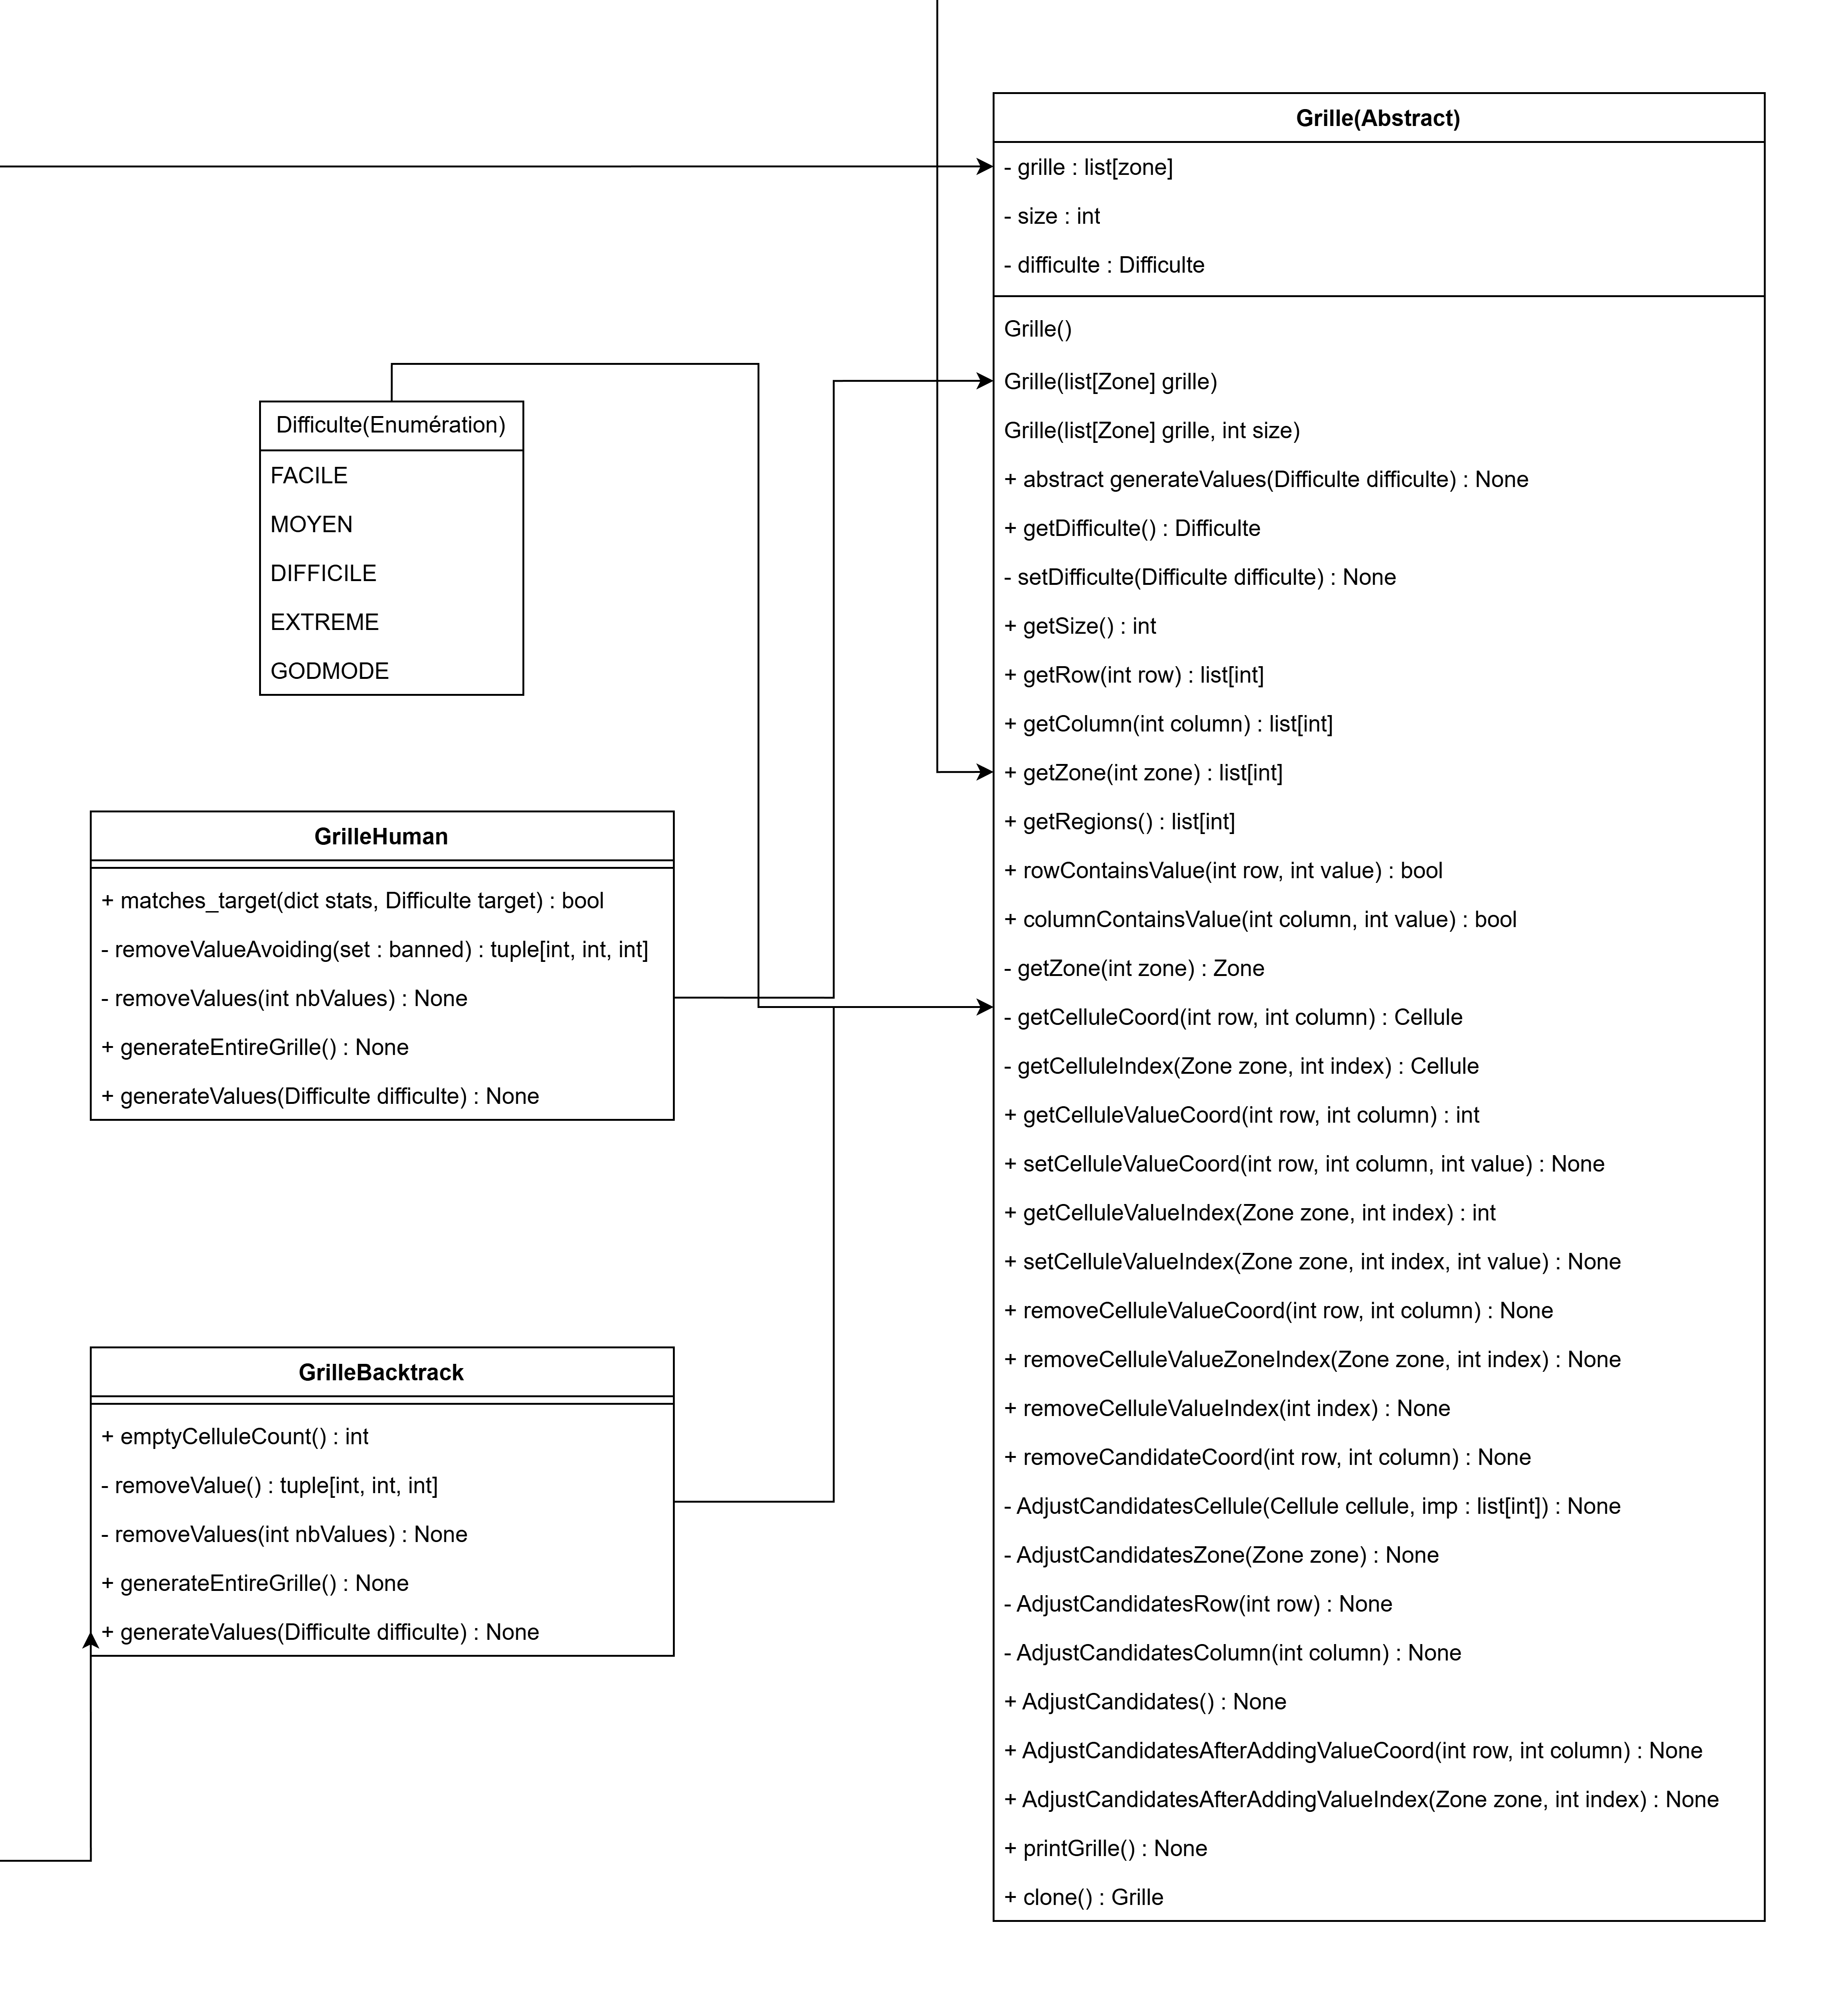
\includegraphics[width=0.65\textwidth]{Diagramme_classe/DiagrammeSlice/Grille_GEN.png}
    \caption{Le diagramme UML représentant les classes des grilles}
    \label{fig:grilleGen}
\end{figure}

\begin{figure}[H]
    \centering
    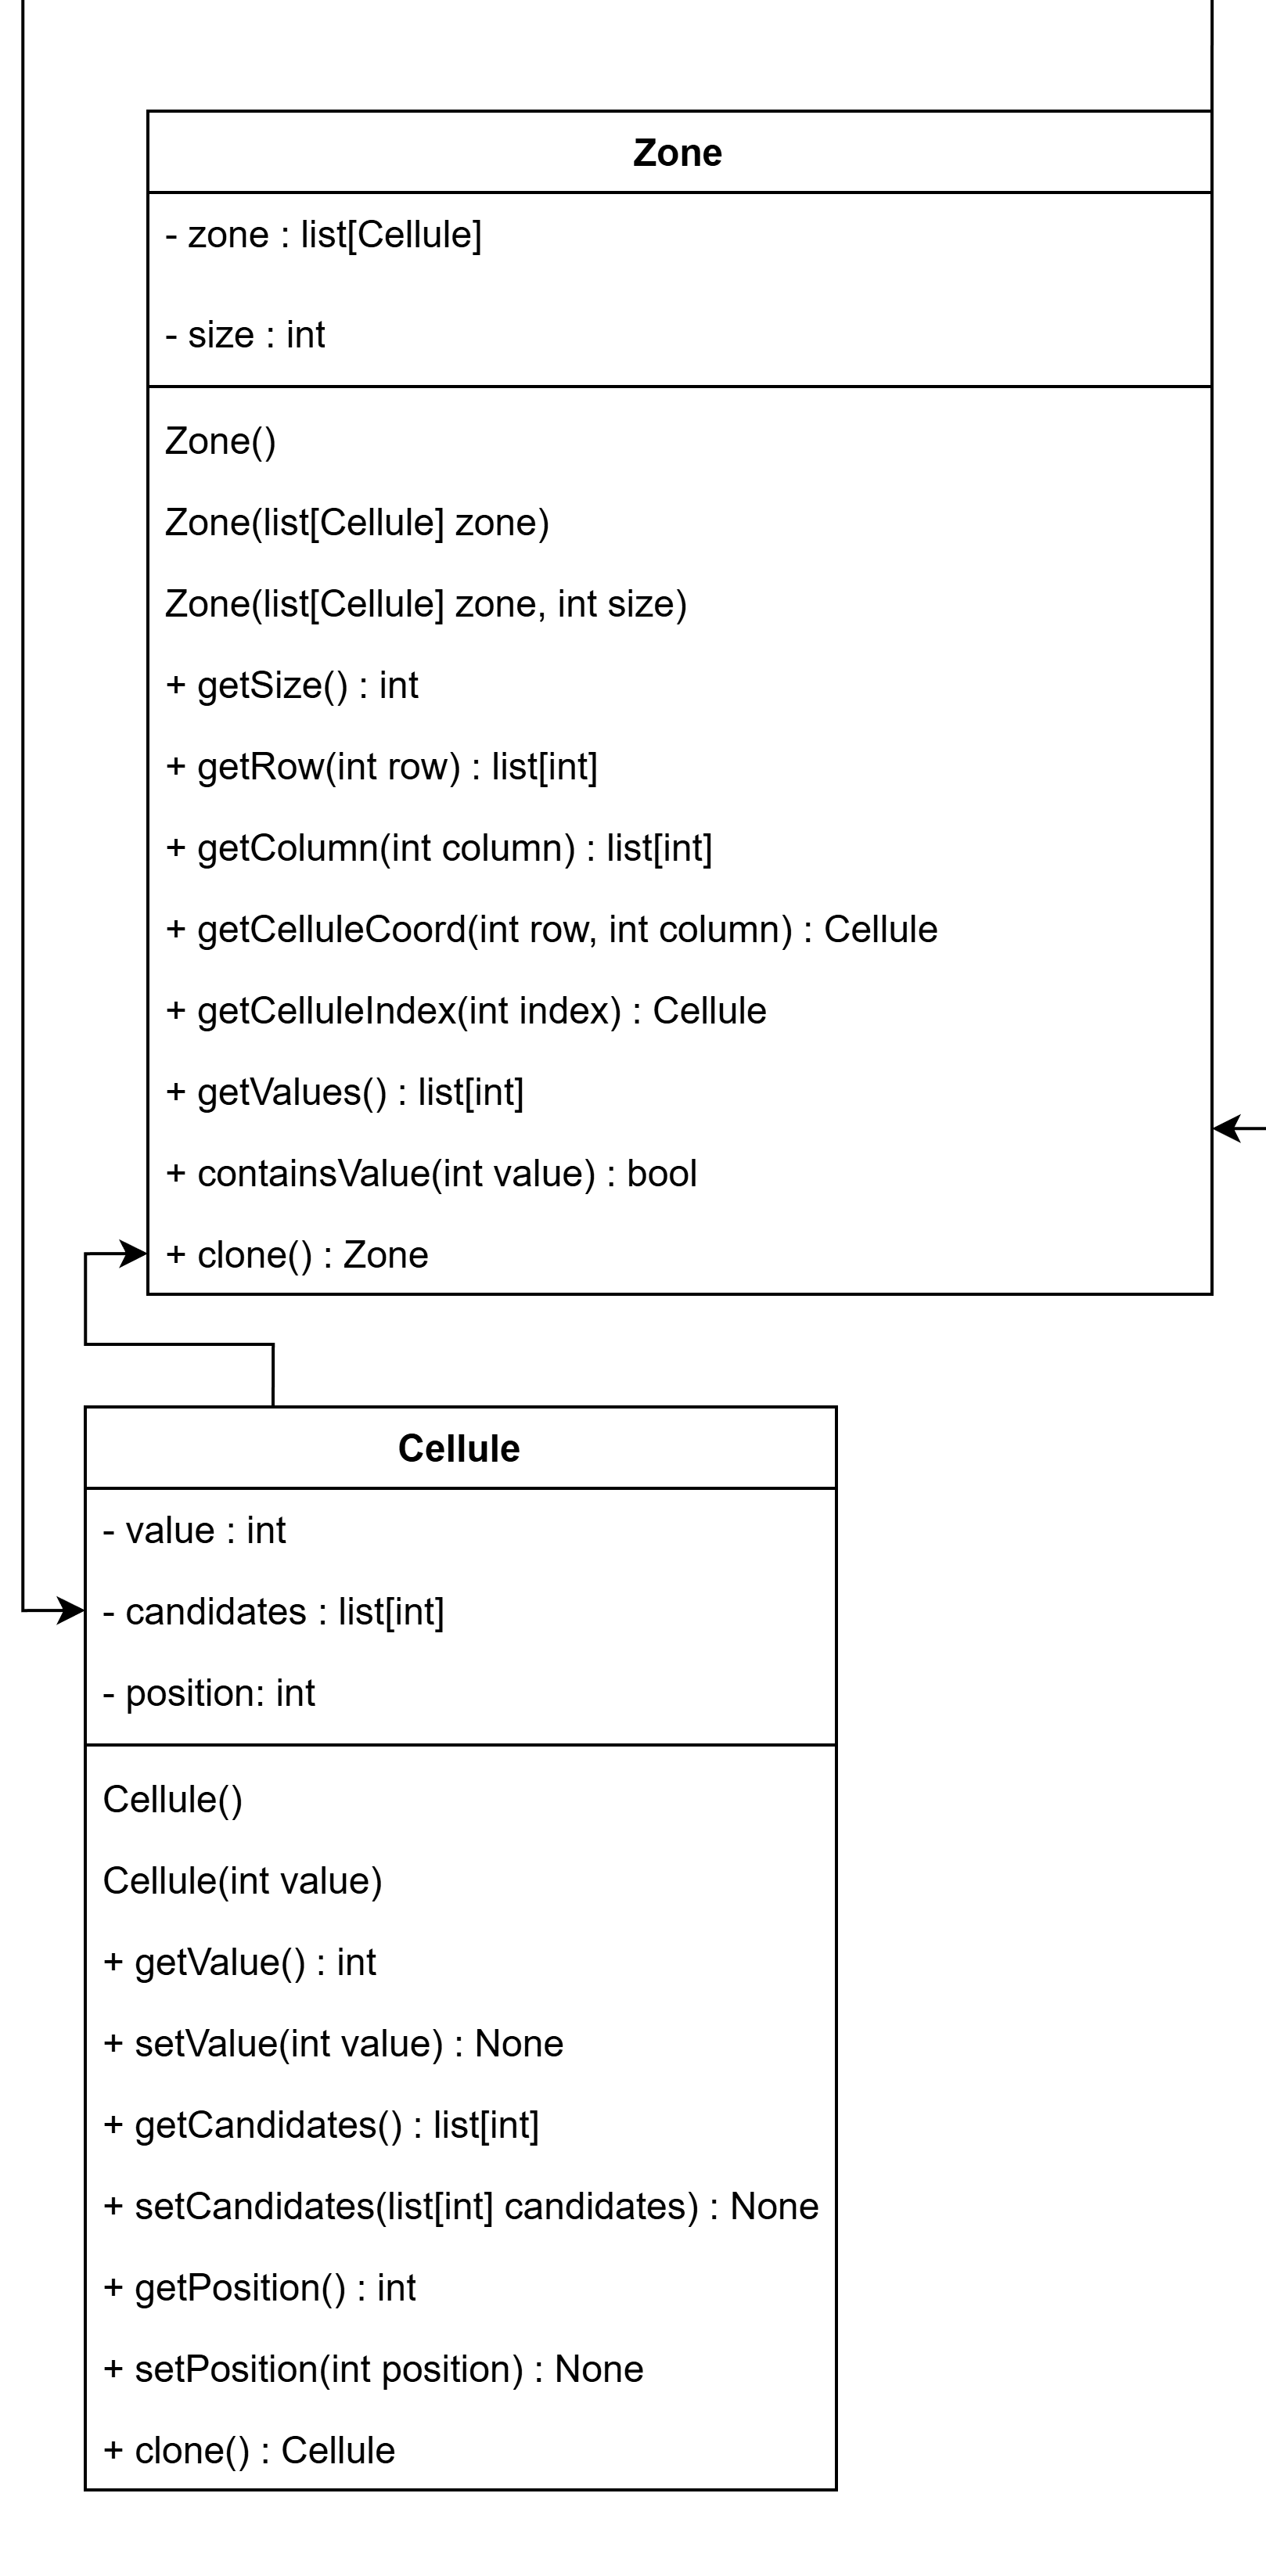
\includegraphics[width=0.55\textwidth]{Diagramme_classe/DiagrammeSlice/Grille_Zone_Cellule.png}
    \caption{Le diagramme UML représentant la classe Zone et Cellule}
    \label{fig:zone-cellule}
\end{figure}

\begin{figure}[H]
    \centering
    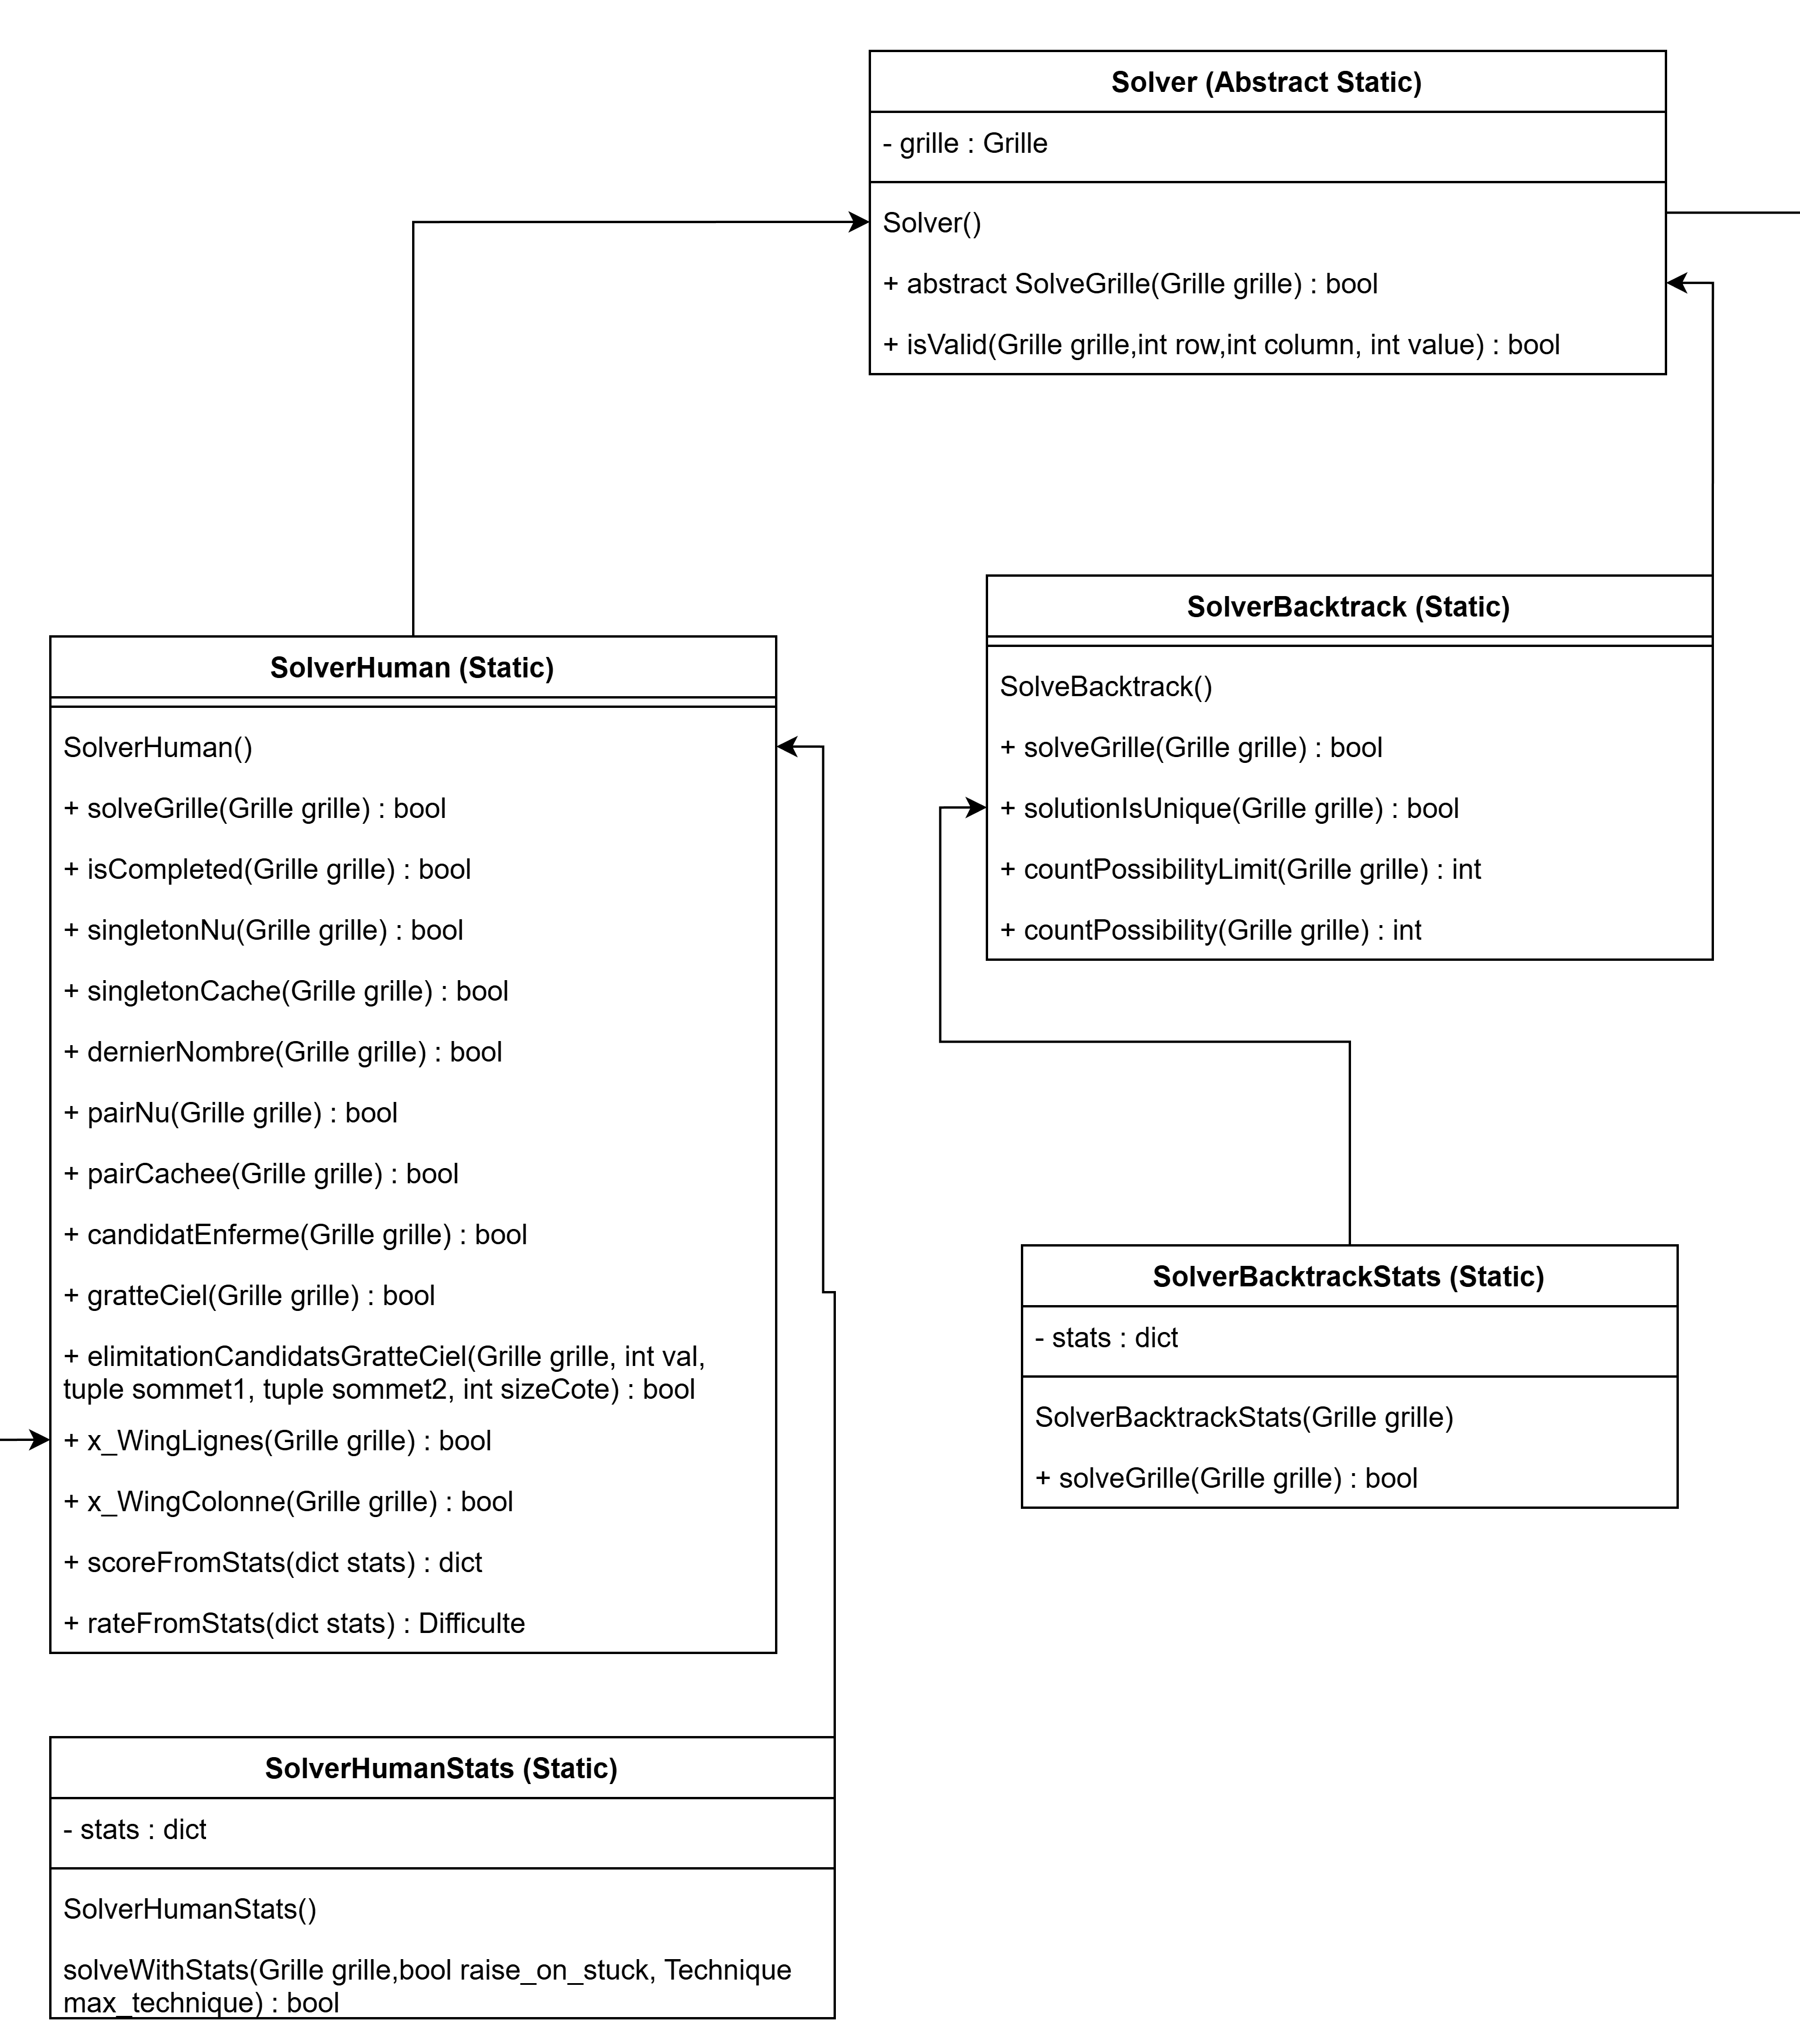
\includegraphics[width=0.60\textwidth]{Diagramme_classe/DiagrammeSlice/Solver.png}
    \caption{Le diagramme UML représentant les classes de Solver}
    \label{fig:solver}
\end{figure}

\begin{figure}[H]
    \centering
    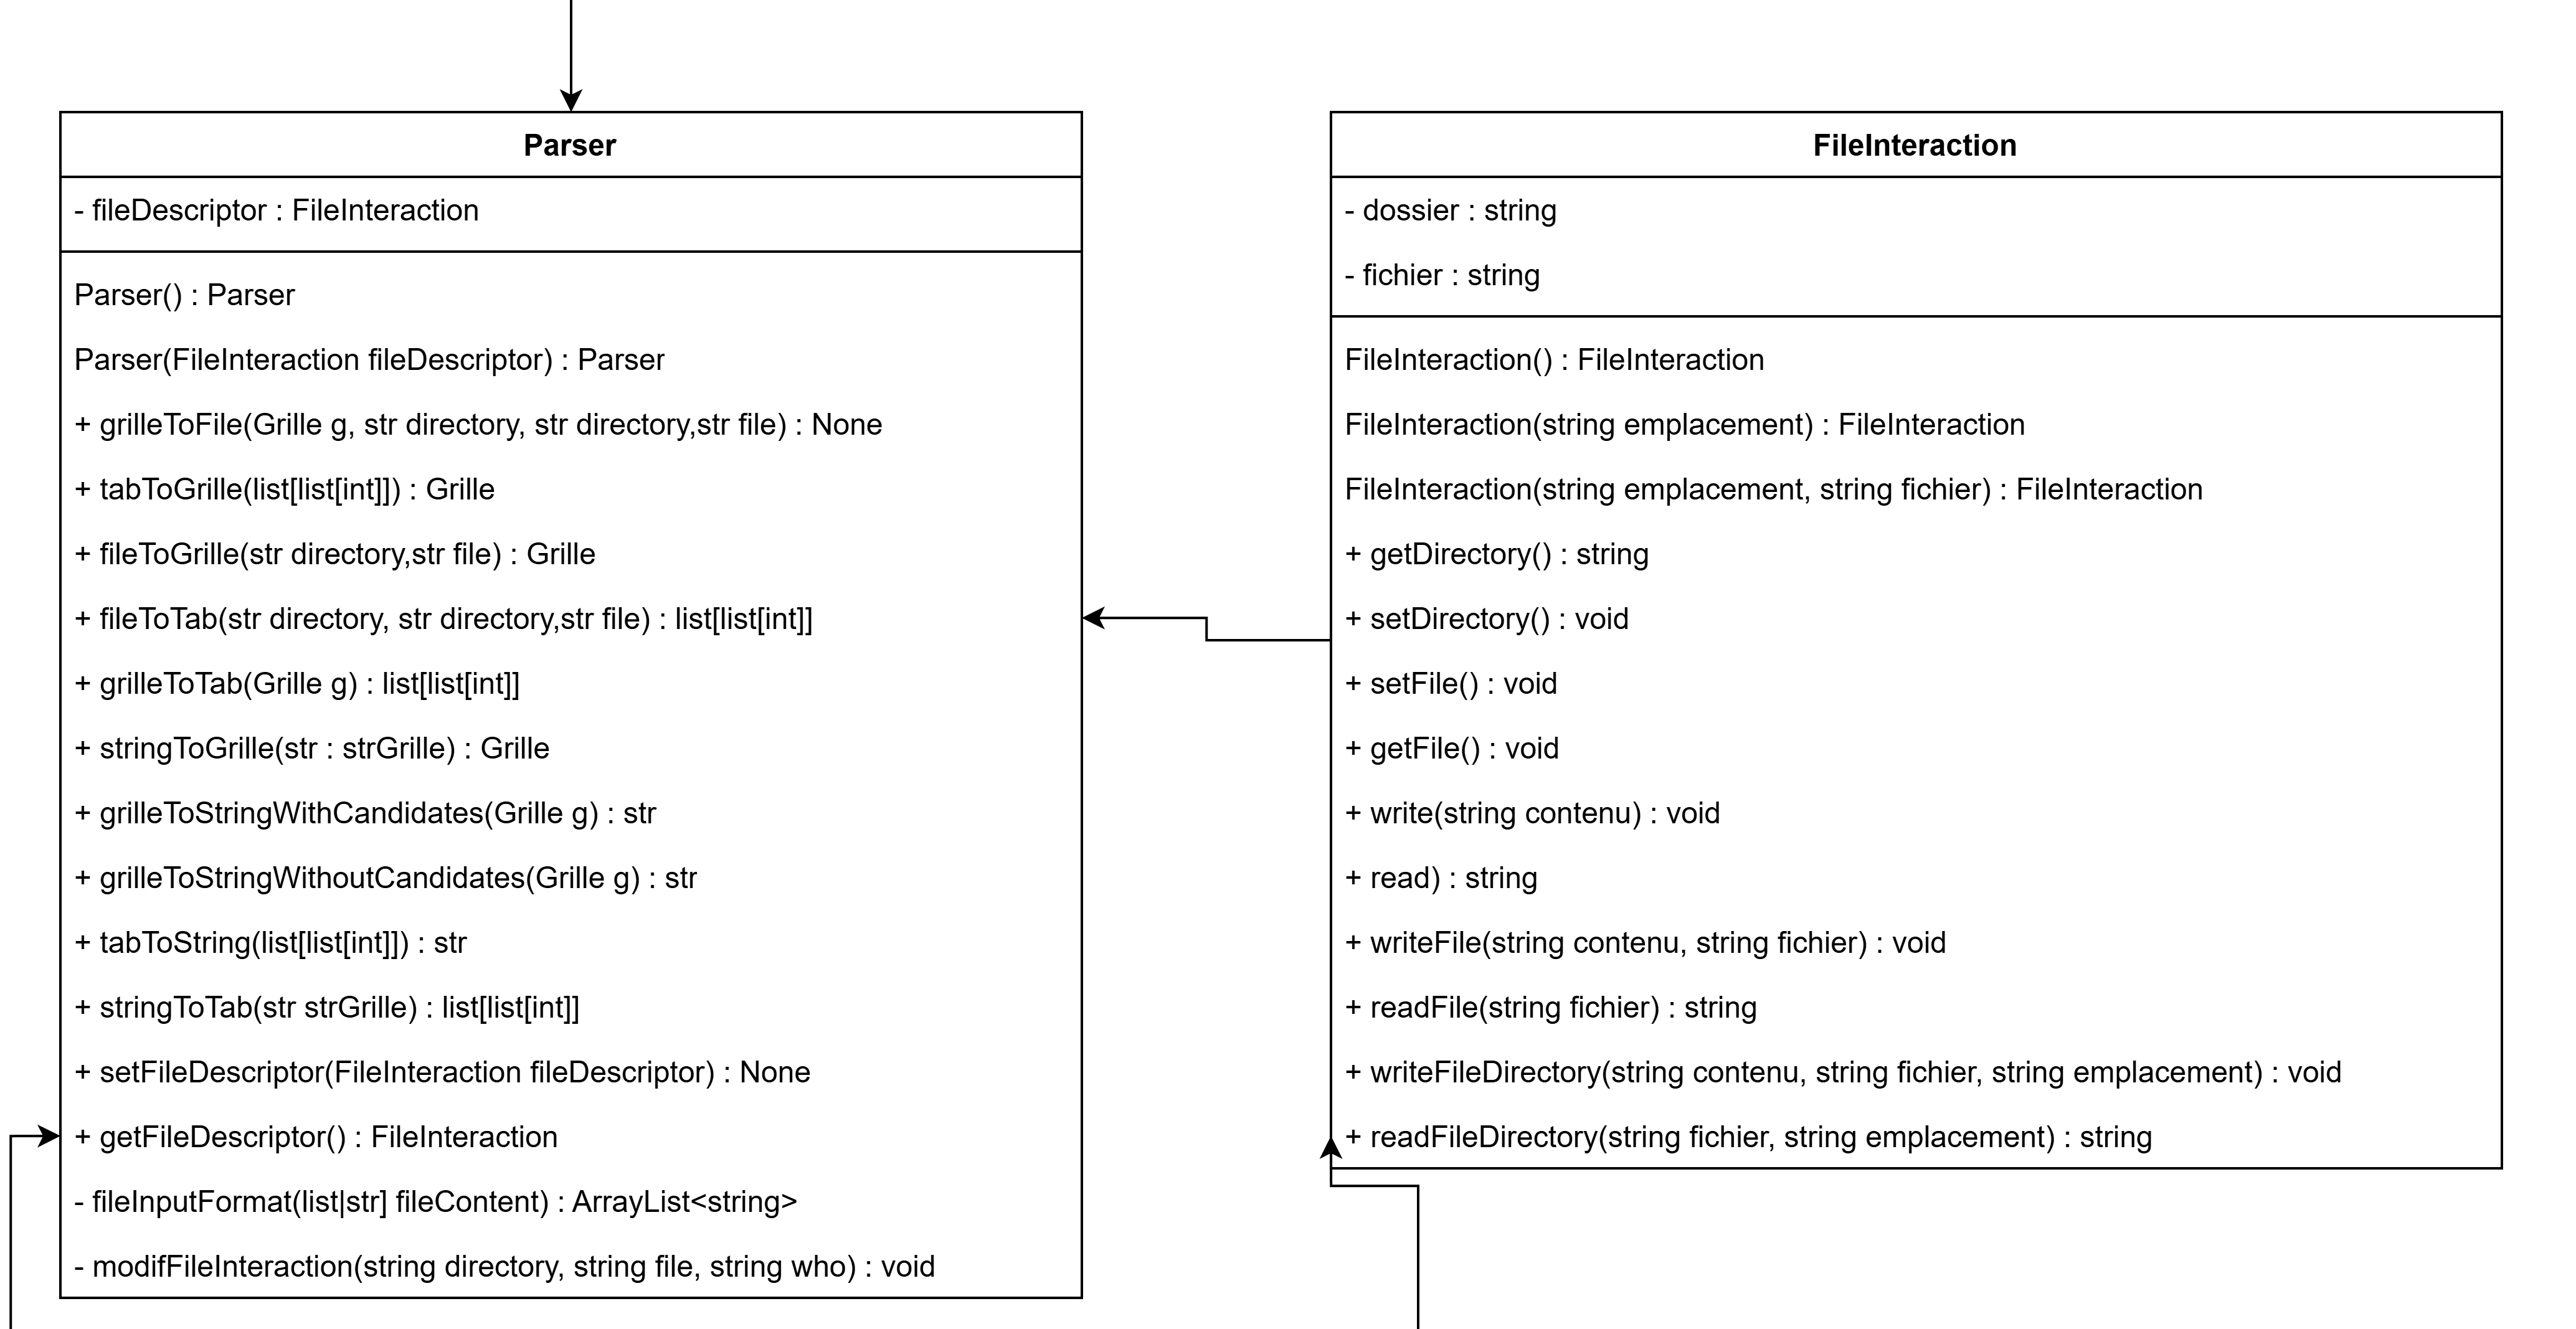
\includegraphics[width=0.60\textwidth]{Diagramme_classe/DiagrammeSlice/Parser.png}
    \caption{Le diagramme UML représentant la classe Parser}
    \label{fig:parser}
\end{figure}

\begin{figure}[H]
    \centering
    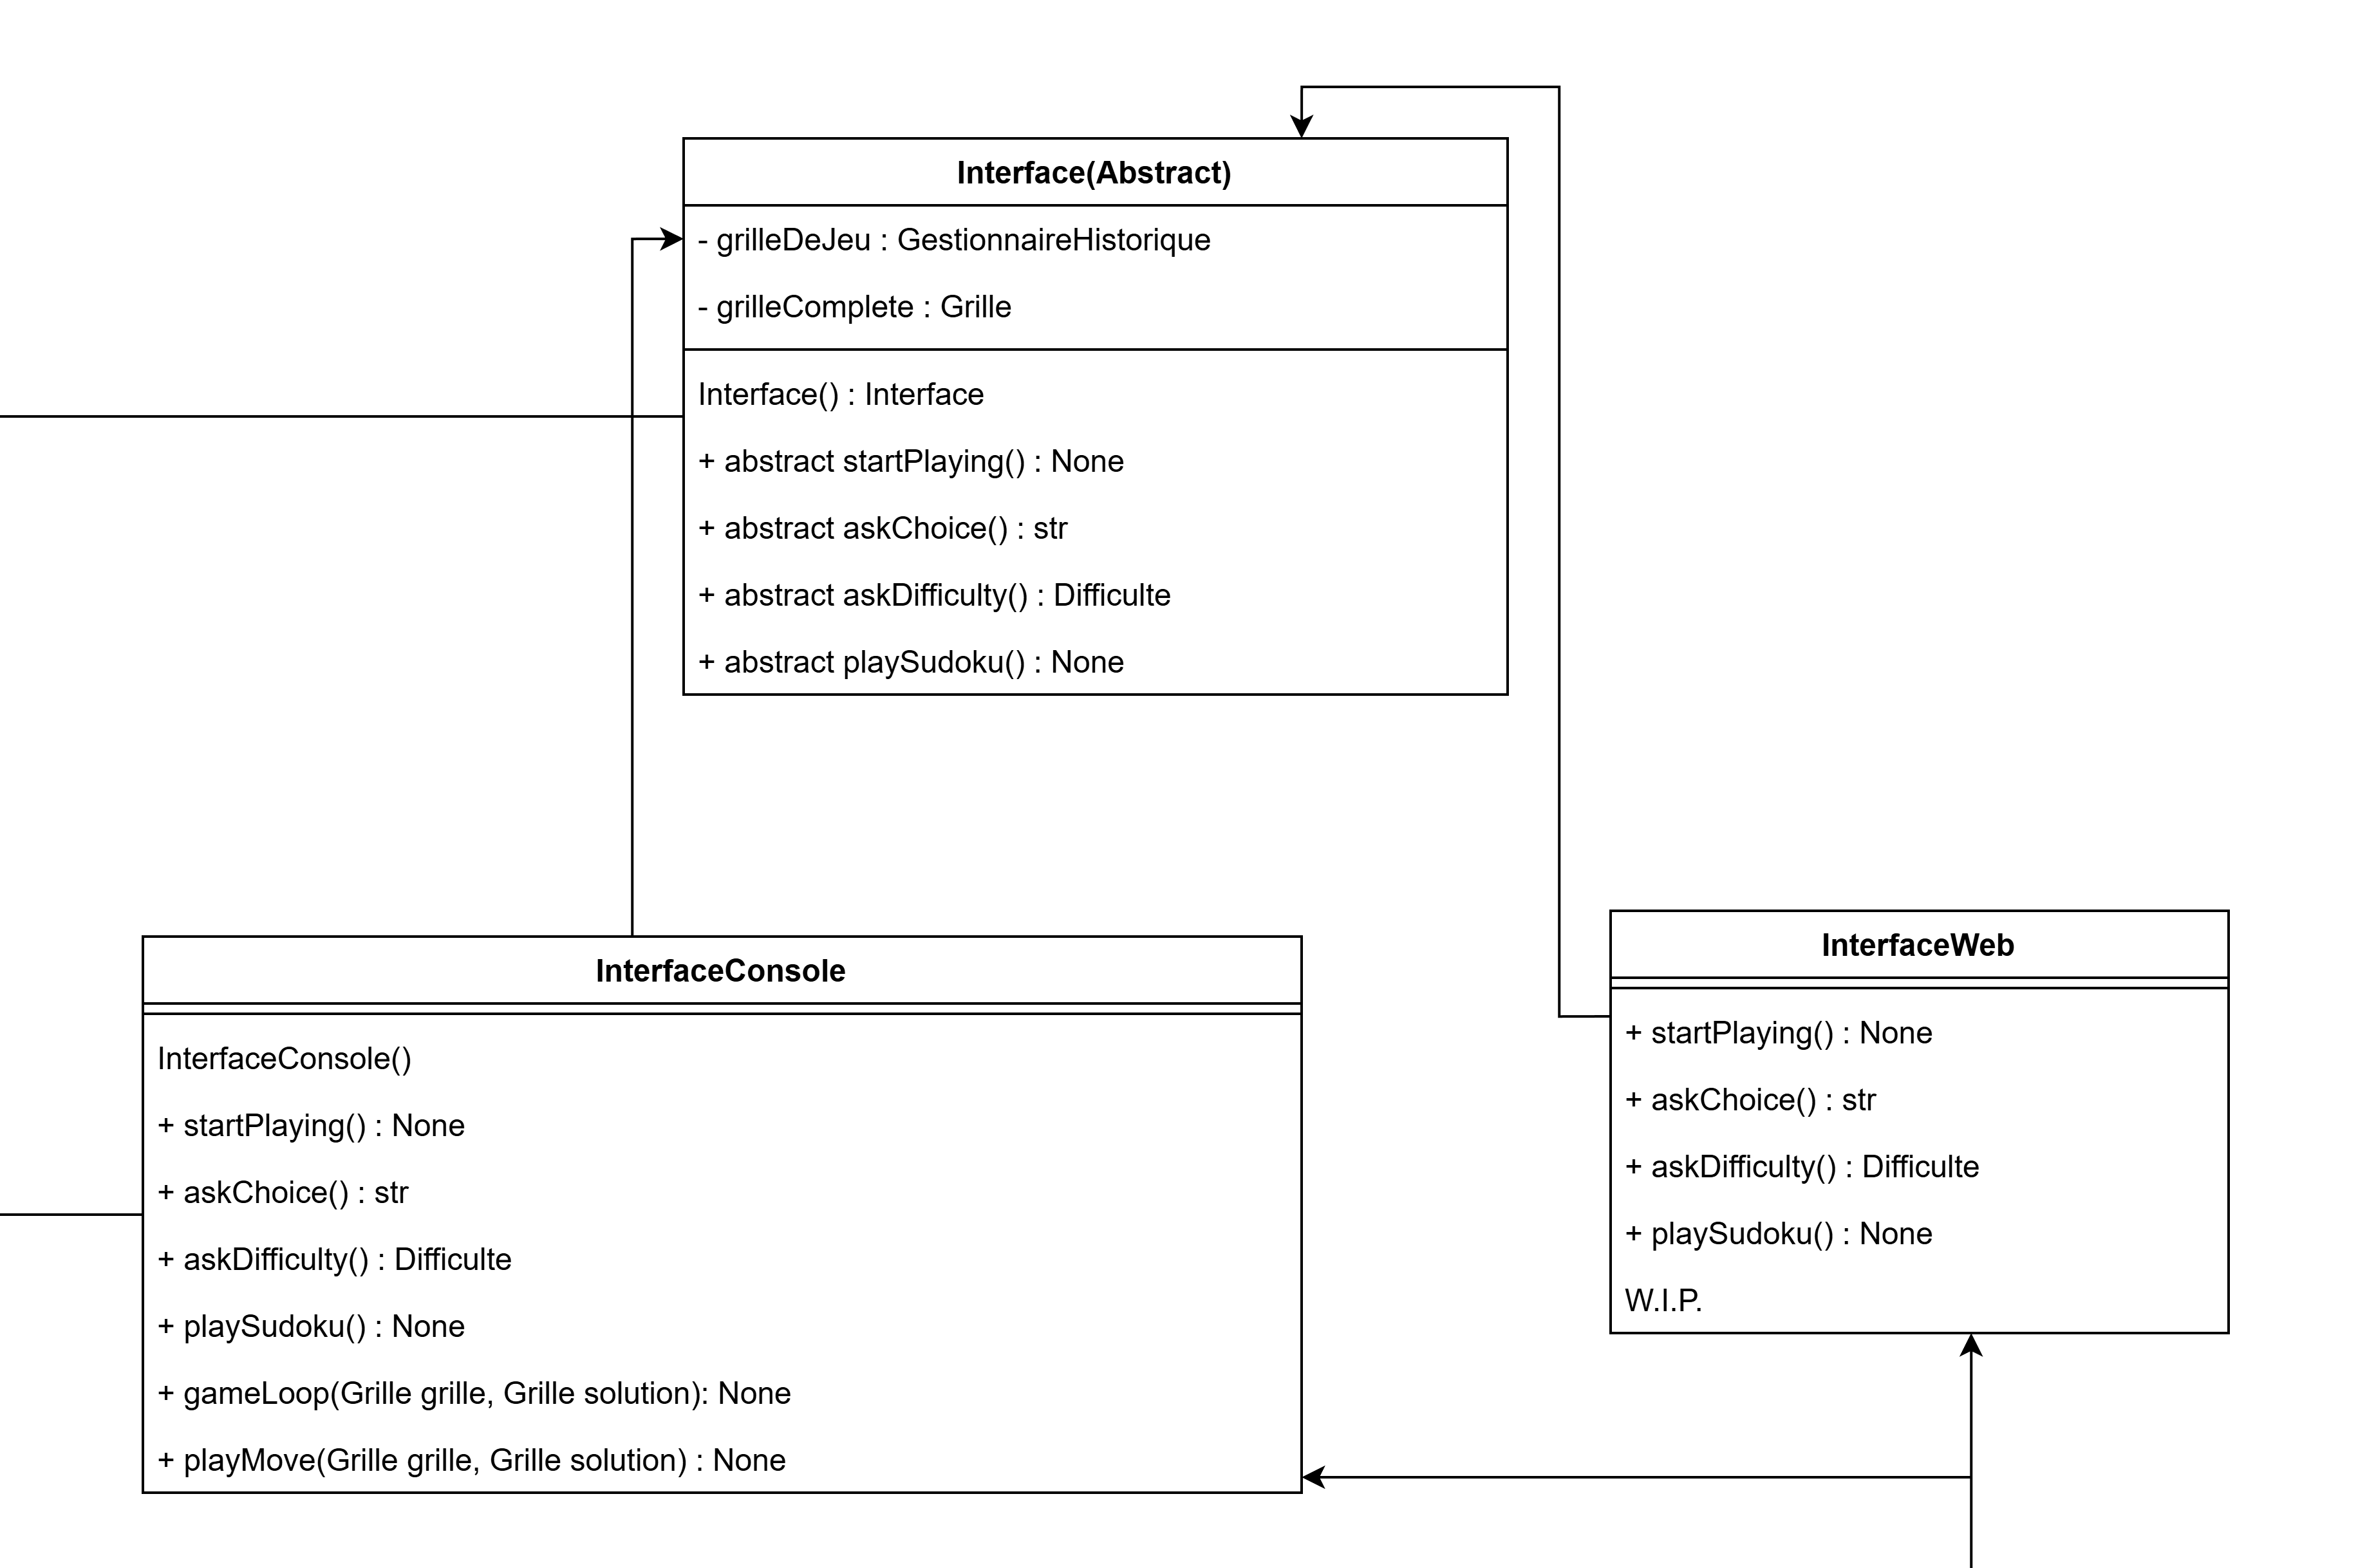
\includegraphics[width=0.60\textwidth]{Diagramme_classe/DiagrammeSlice/Interface.png}
    \caption{Le diagramme UML représentant les classes d'Interface}
    \label{fig:interface}
\end{figure}

\begin{figure}[H]
    \centering
    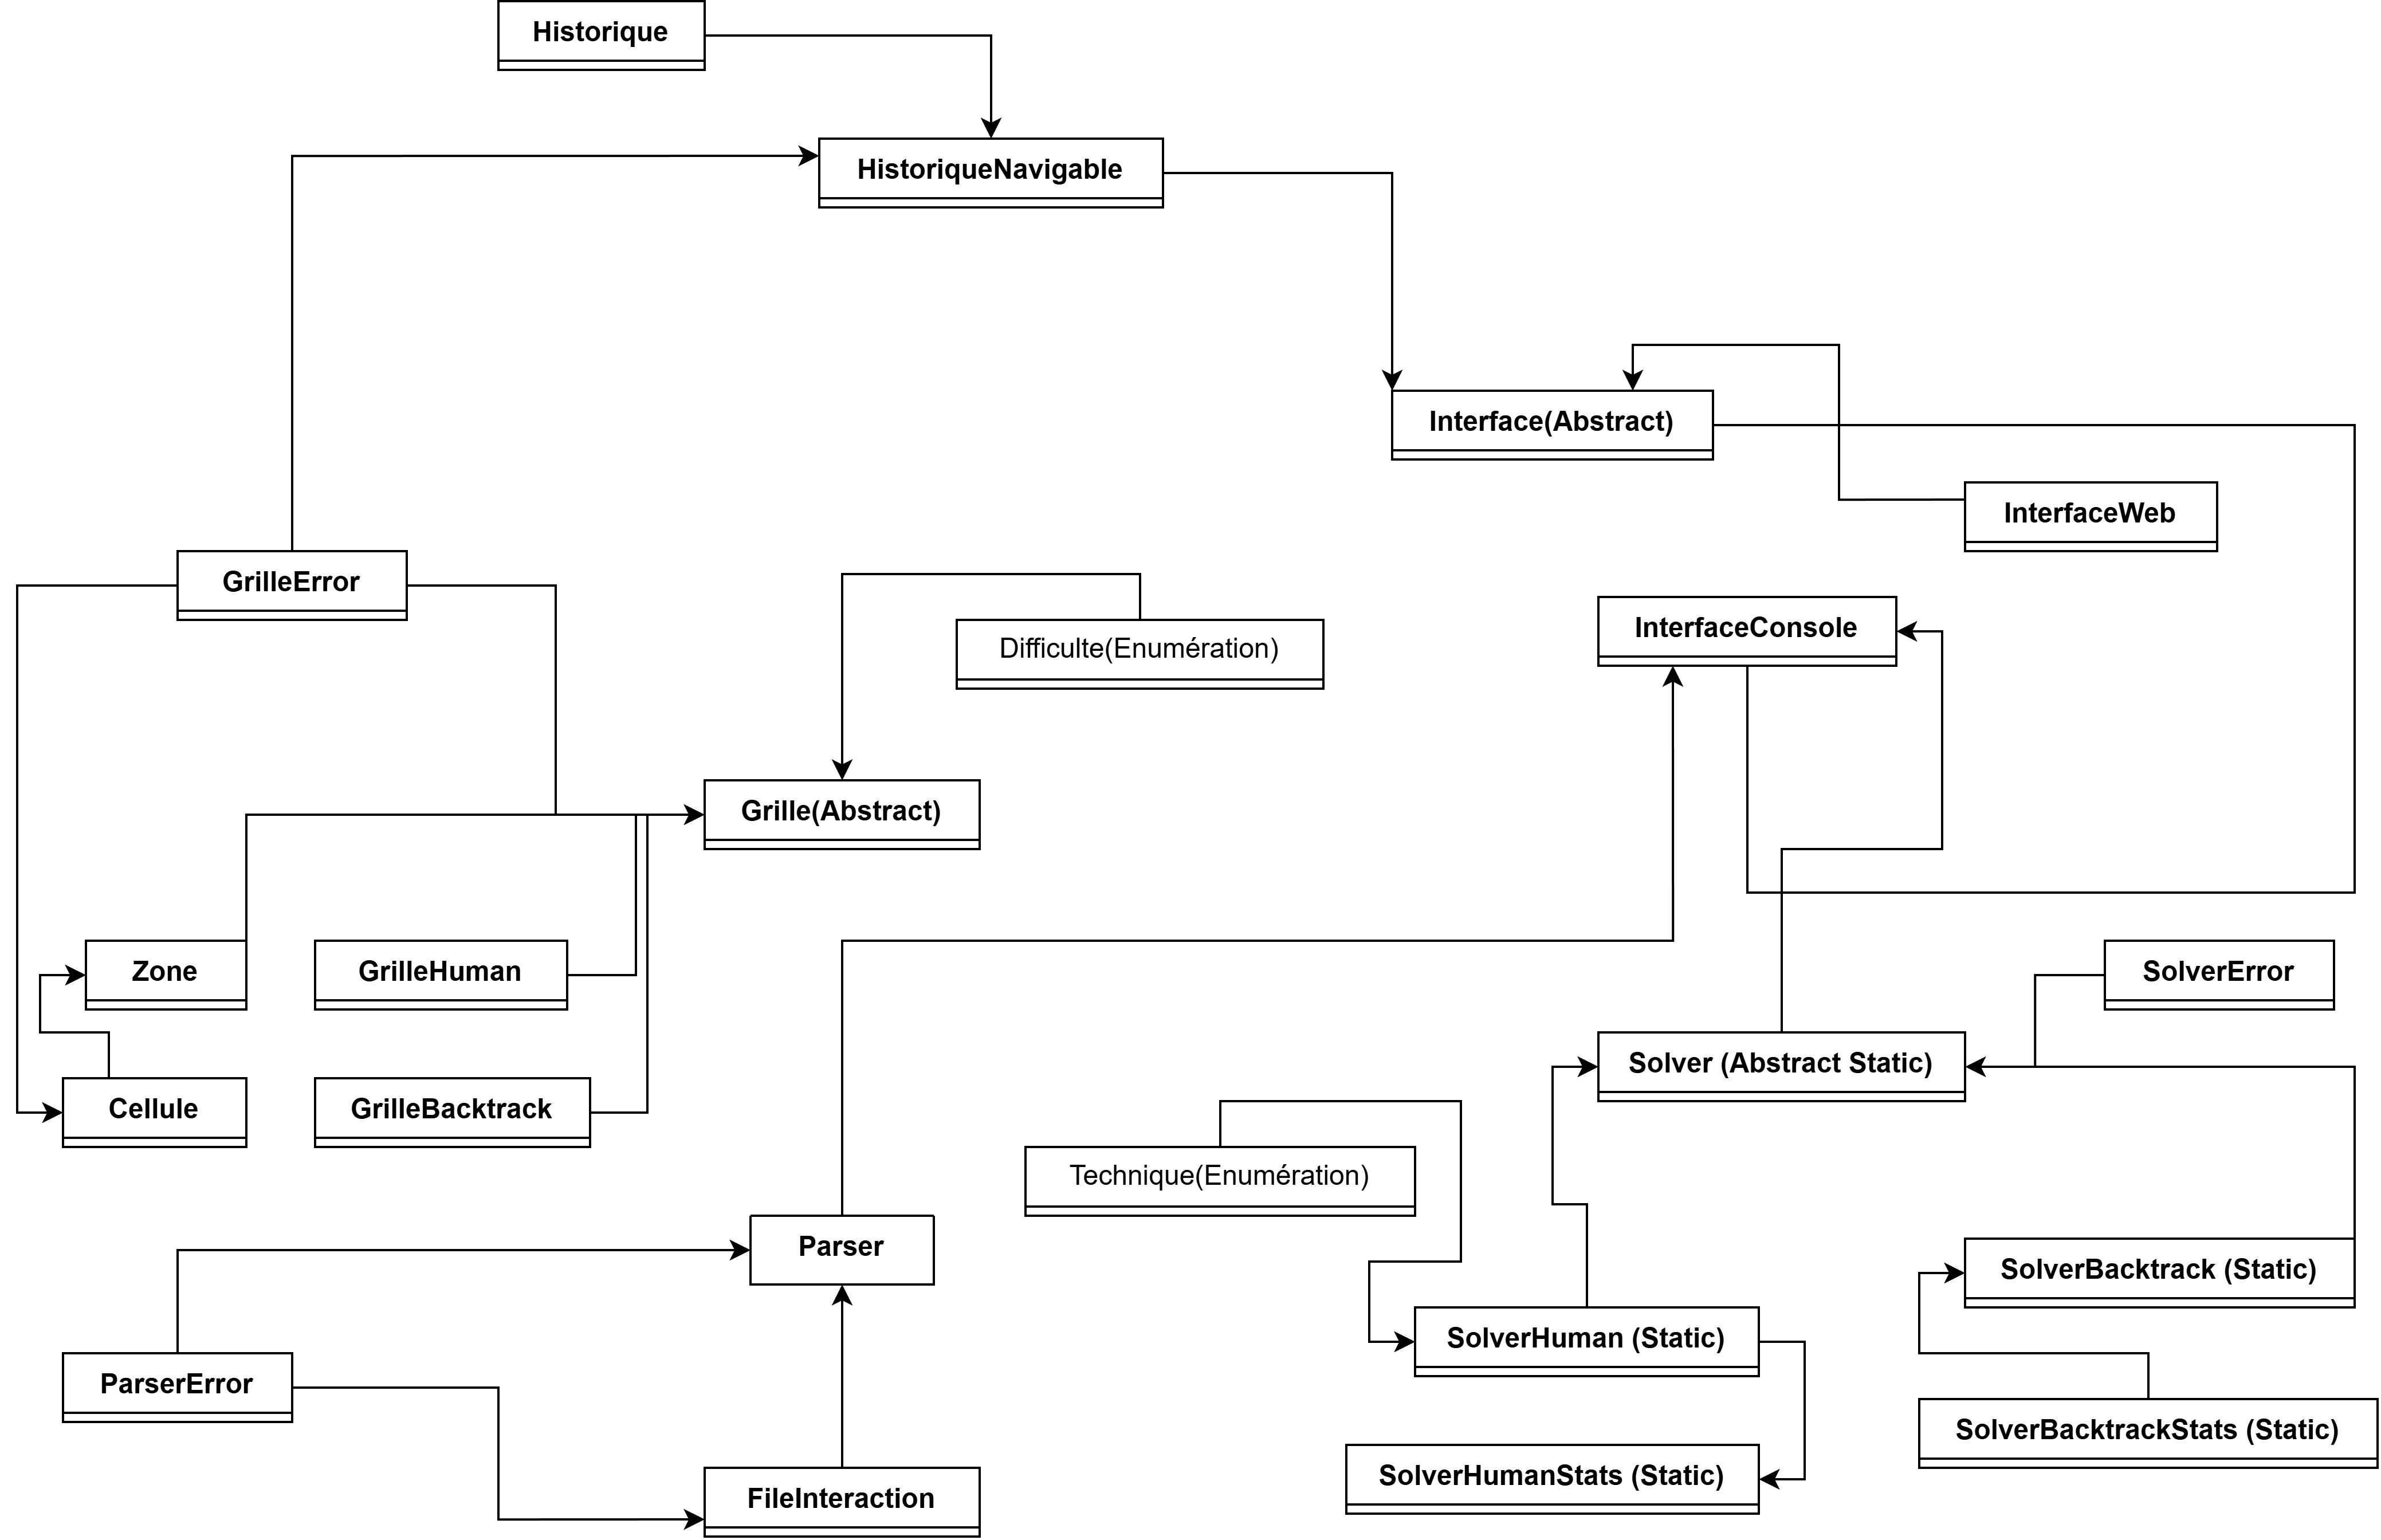
\includegraphics[width=0.60\textwidth]{Diagramme_classe/Diagramme_simpl.png}
    \caption{Le diagramme UML entier et simplifié}
    \label{fig:UML}
\end{figure}

\begin{figure}[H]
    \centering
    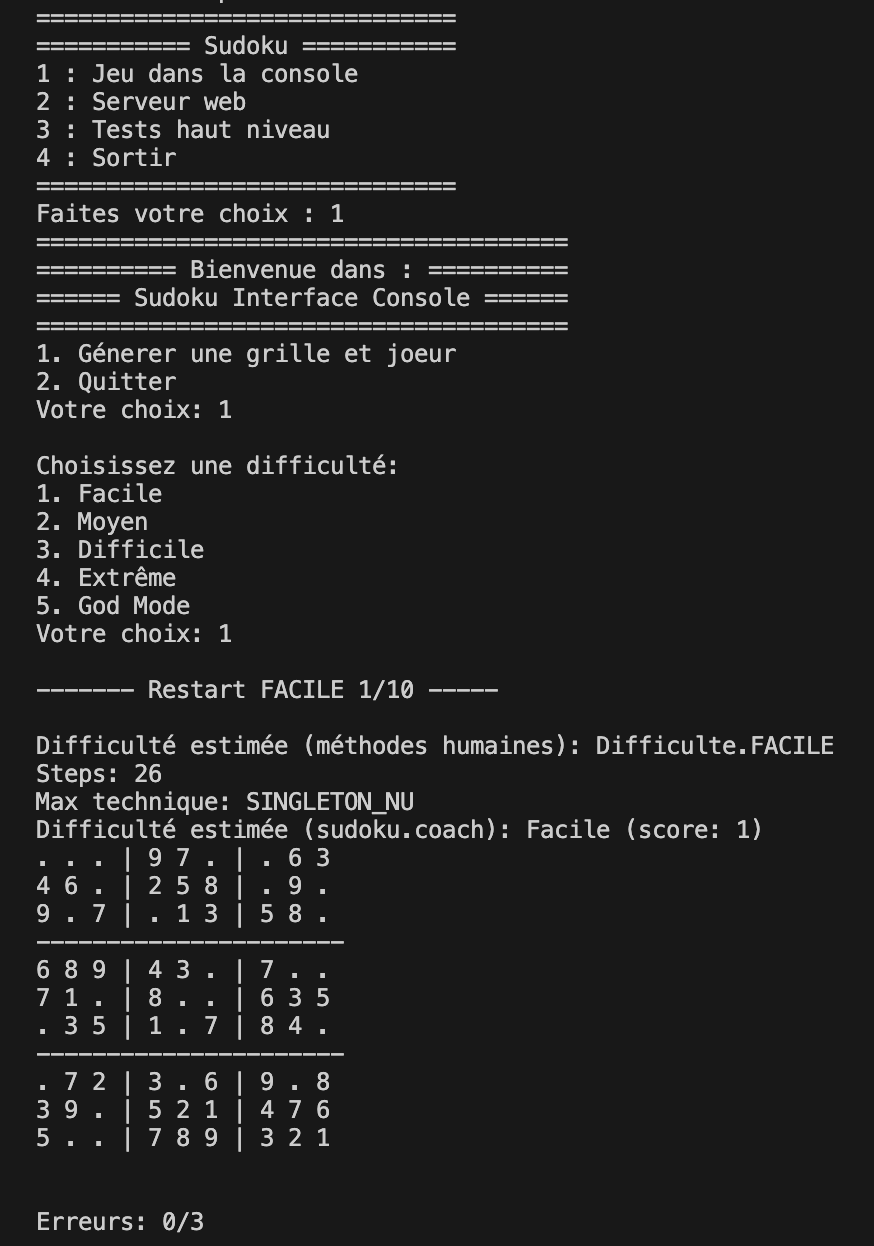
\includegraphics[width=0.60\textwidth]{grilleFacile.png}
    \caption{Exemple d'une grille facile affichée dans l'interface console}
    \label{fig:grille-facile}
\end{figure}

\begin{figure}[H]
    \centering
    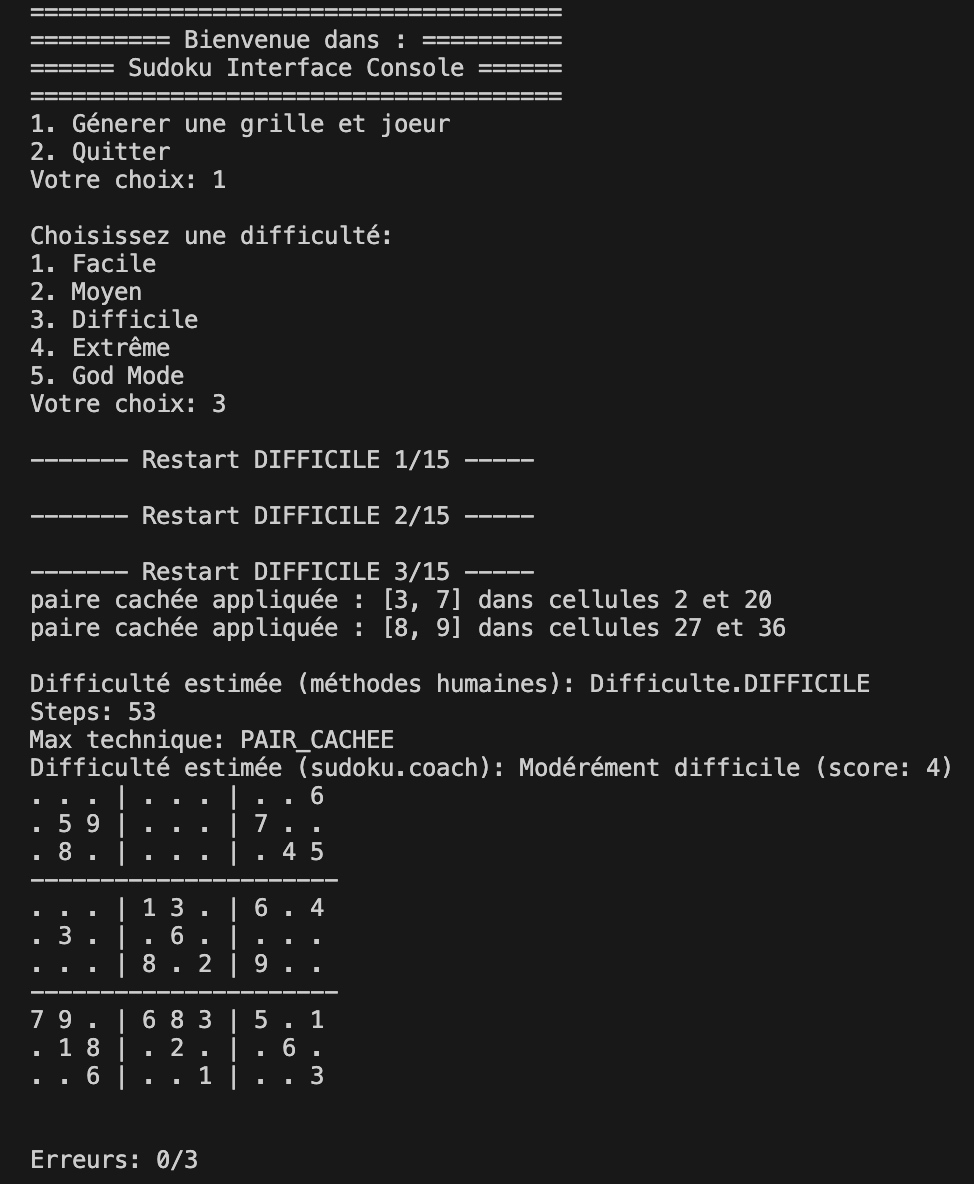
\includegraphics[width=0.70\textwidth]{grilleDifficile.png}
    \caption{Exemple d'une grille difficile affichée dans l'interface console}
    \label{fig:grille-difficile}
\end{figure}

\begin{figure}[H]
    \centering
    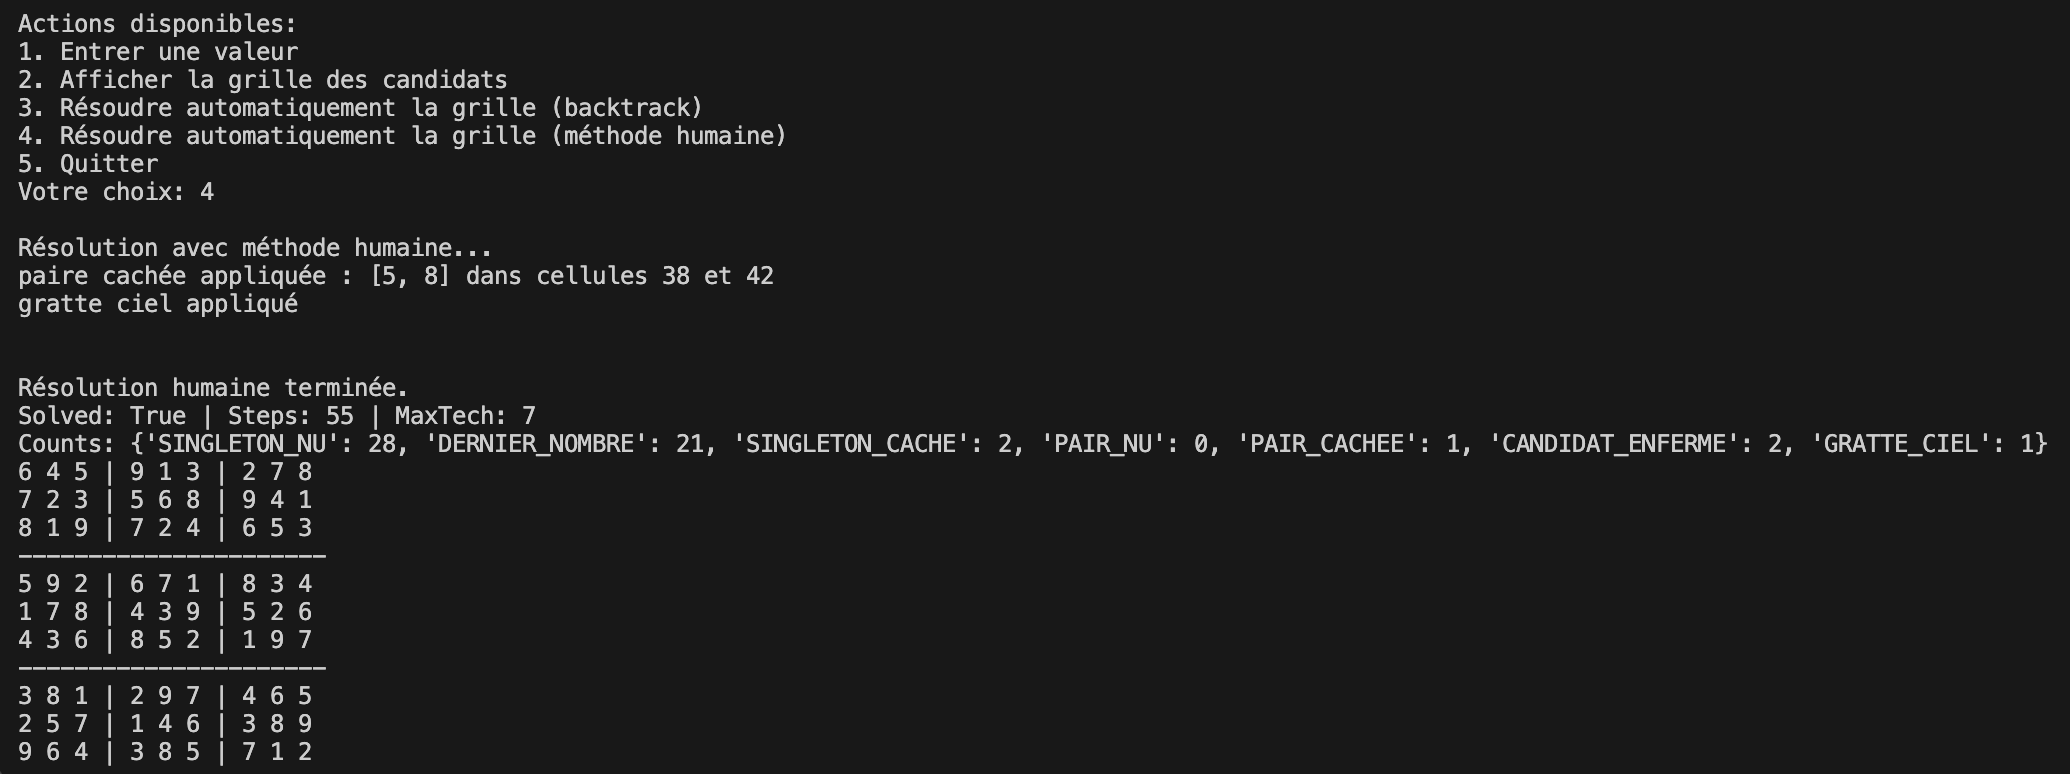
\includegraphics[width=0.80\textwidth]{grilleExtremeResolu.png}
    \caption{Exemple d'une grille extrême résolue avec des techniques humaines dans l'interface console}
    \label{fig:grille-extreme-resolu}
\end{figure}

\begin{figure}[H]
    \centering
    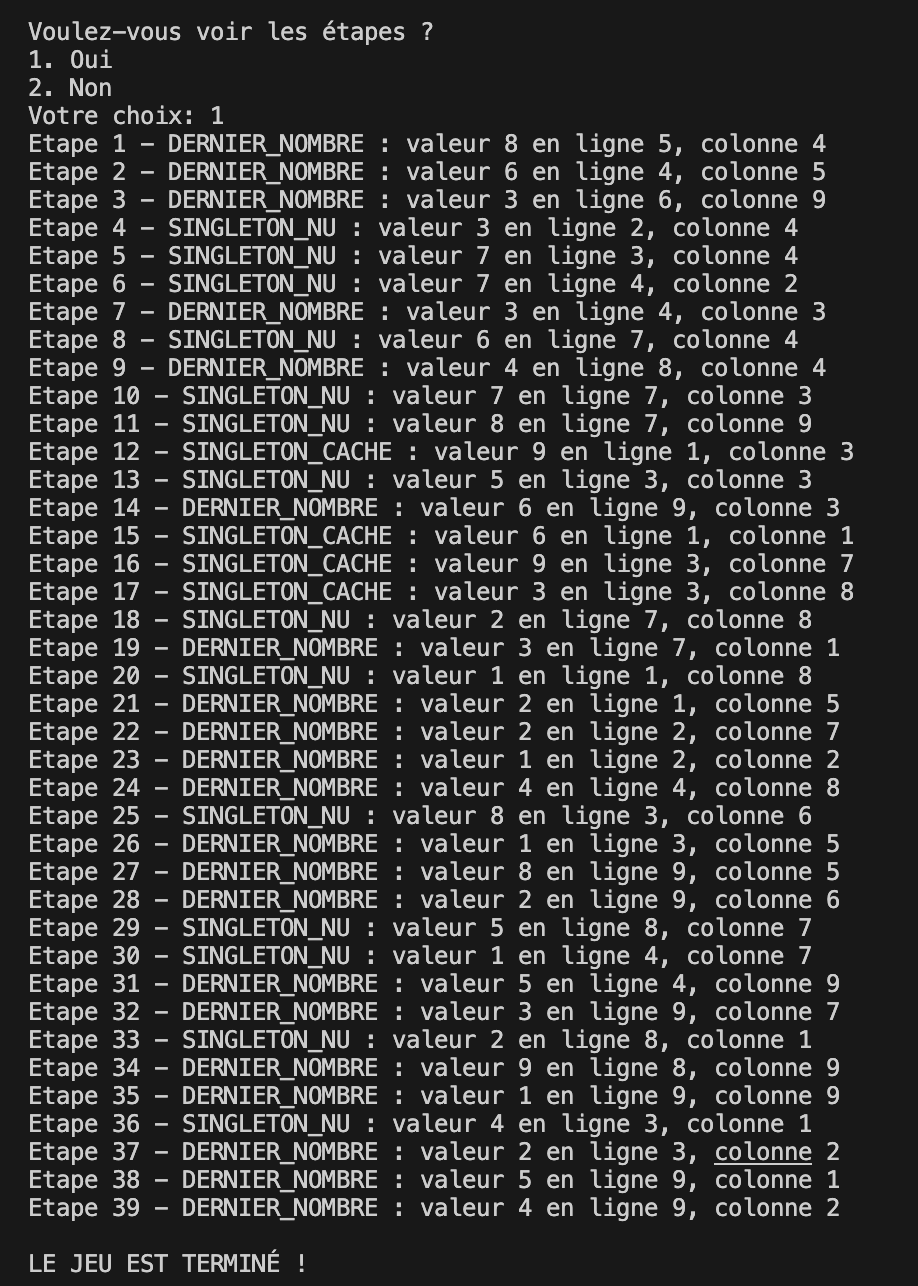
\includegraphics[width=0.60\textwidth]{etapesMoyen.png}
    \caption{Exemple des étapes d'une grille moyen resolue avec des techniques humaines dans l'interface console}
    \label{fig:etapes-moyen}
\end{figure}

\begin{figure}[H]
    \centering
    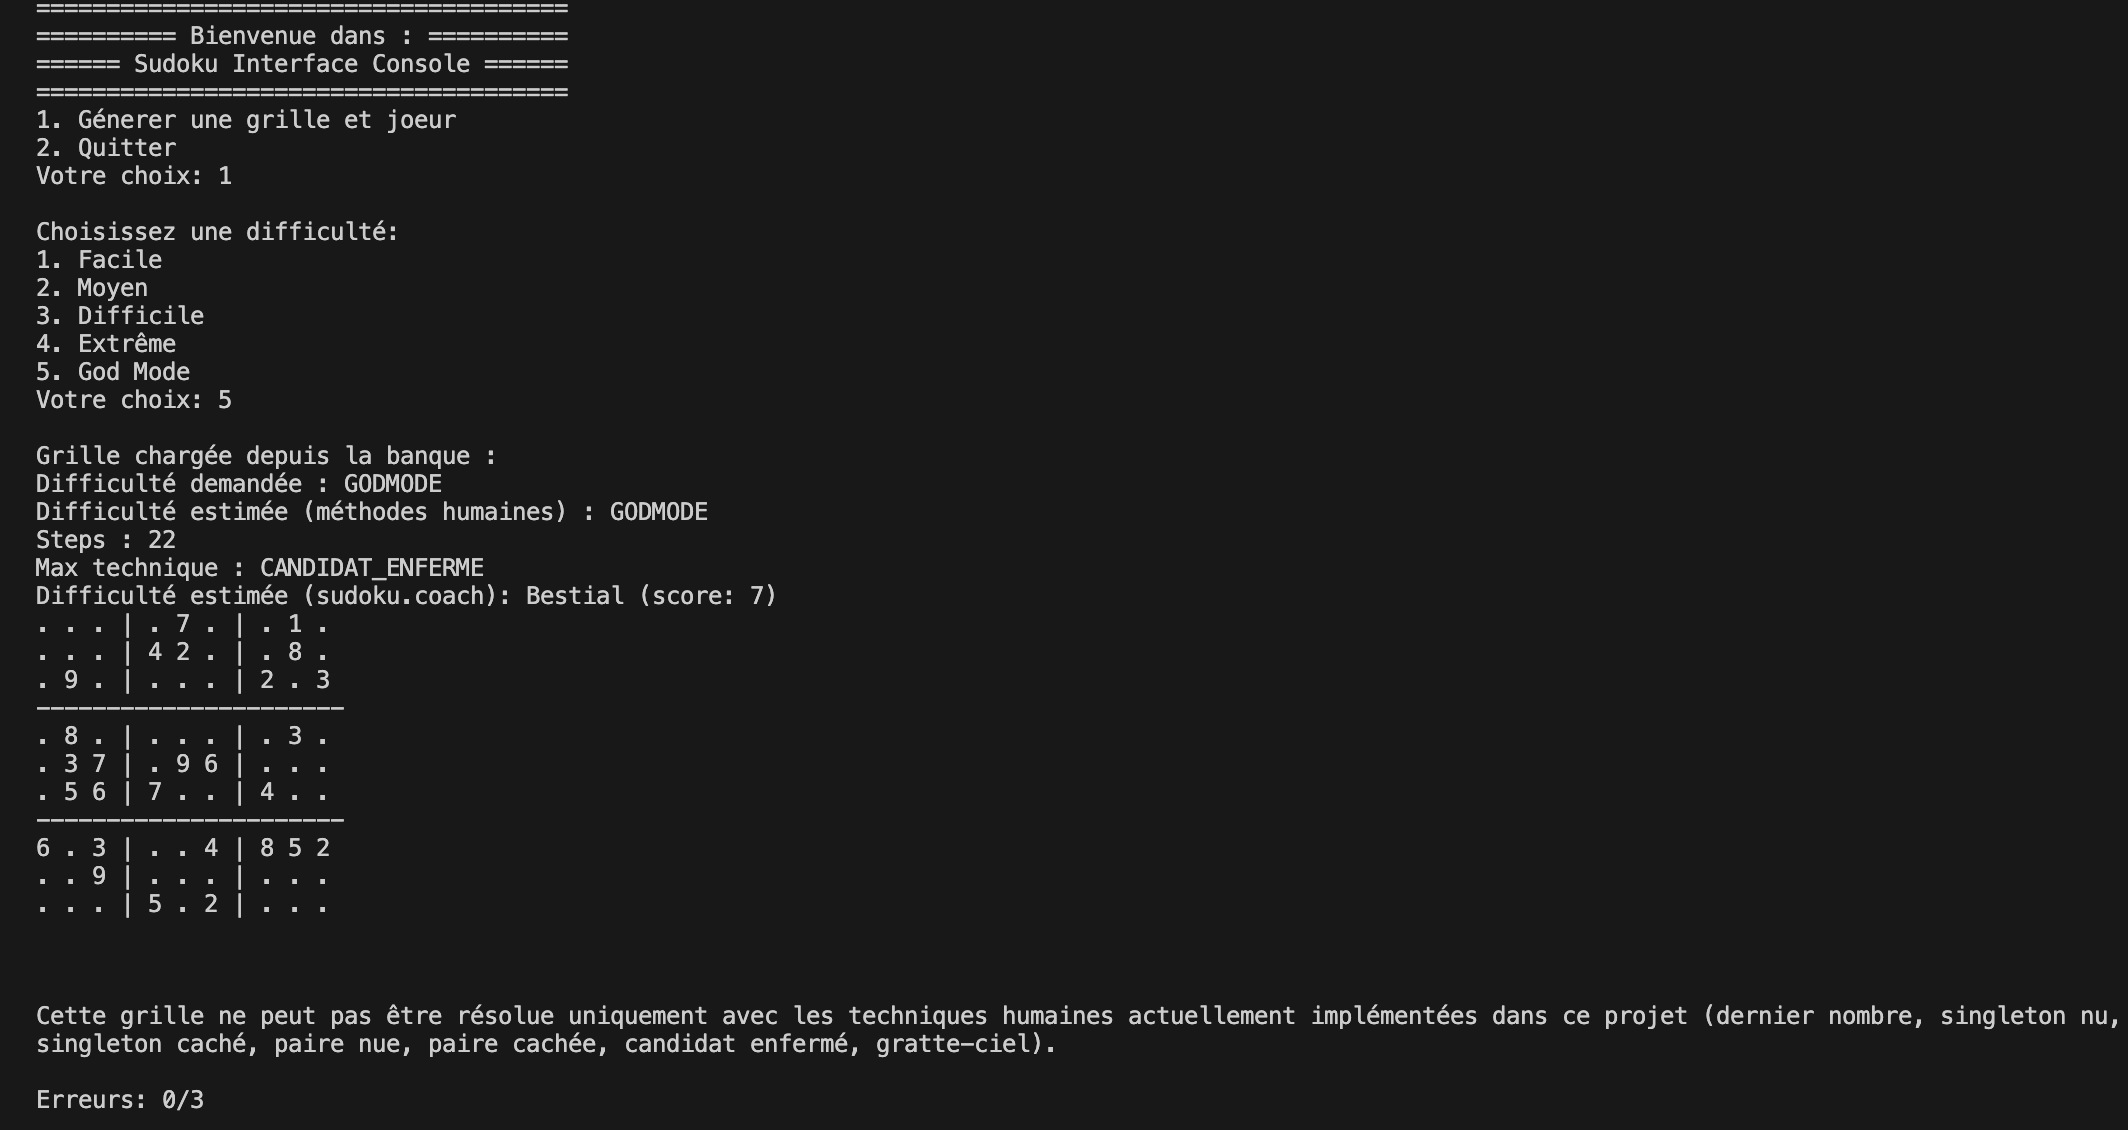
\includegraphics[width=0.78\textwidth]{grilleGodmodeBanque.png}
    \caption{Chargement d'une grille GodMode depuis la banque de grilles pré-générées}
    \label{fig:grille-godmode}
\end{figure}



\end{document}